\documentclass[11pt, a4paper]{jarticle}
% \usepackage{../style/new_coe}
%\usepackage{../style/coe}
\usepackage[dvipdfmx]{graphicx}
\usepackage{wrapfig}
\usepackage{bm}
\usepackage{amsmath, amssymb}
\usepackage{type1cm}
\usepackage{docmute}
\renewcommand{\figurename}{Fig.}
\renewcommand{\tablename}{Table }
\usepackage{caption, subcaption}
\usepackage{comment}

\topmargin=-.4mm
\oddsidemargin=-0.4mm \evensidemargin=\oddsidemargin
\setlength{\textwidth}{160mm}
\usepackage{algorithmic}
\usepackage{algorithm}

% TITLE of the article
\title{すんすんアルバイト登録の説明書}

% AUTHOR name
\author{金栄世}

%----------------------------------------------------------------------

\begin{document}
\maketitle

\section{社員/従業員共通の操作}
	\subsection{ログイン画面}
		\begin{figure}[htbp]
			\centering
			\fbox{
					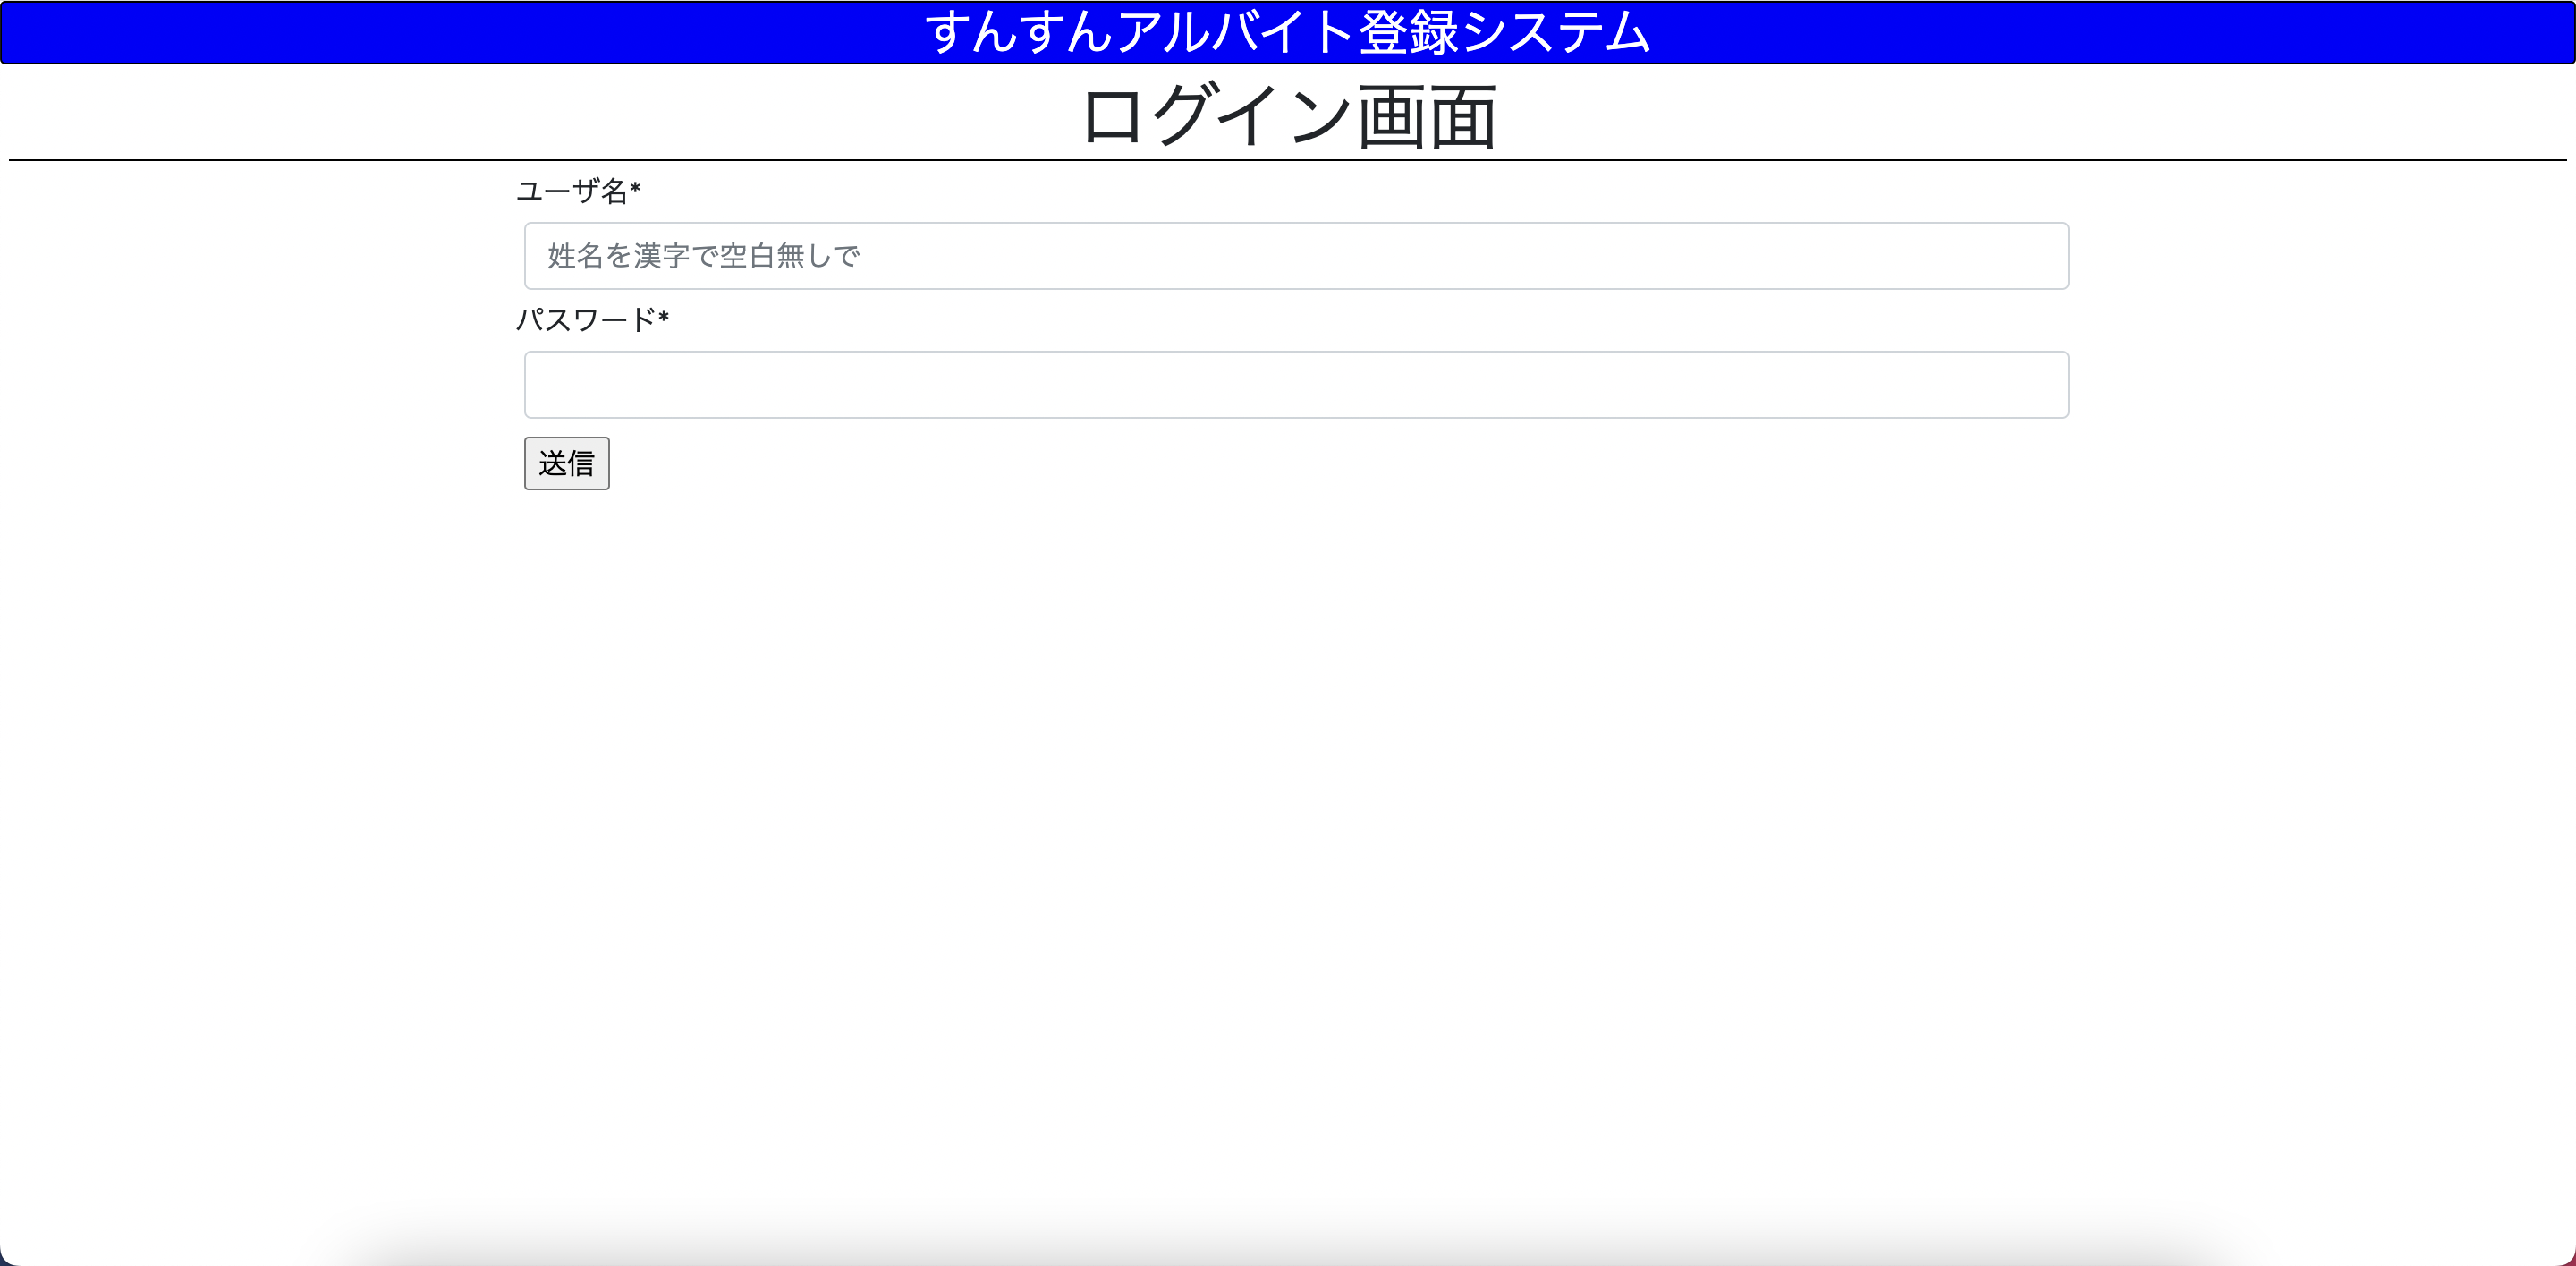
\includegraphics[width=0.8\linewidth]{../figure/1_login.png}
				}
		\end{figure}
		この画面ではログインを行います。
		名前とパスワードの両方について、登録されている情報と完全に一致した場合に認証を行っています。
		尚、ログインしていない状態で他のページにアクセスしようとした際にはこのページに強制的に飛ばされるように設定されています。
		このアプリではブラウザの設定にもよりますが、基本的には一度ログインすれば認証はずっと継続されるようになっています。
		\clearpage

	\subsection{登録情報変更画面}
		\begin{figure}[htbp]
				\centering
				\fbox{
						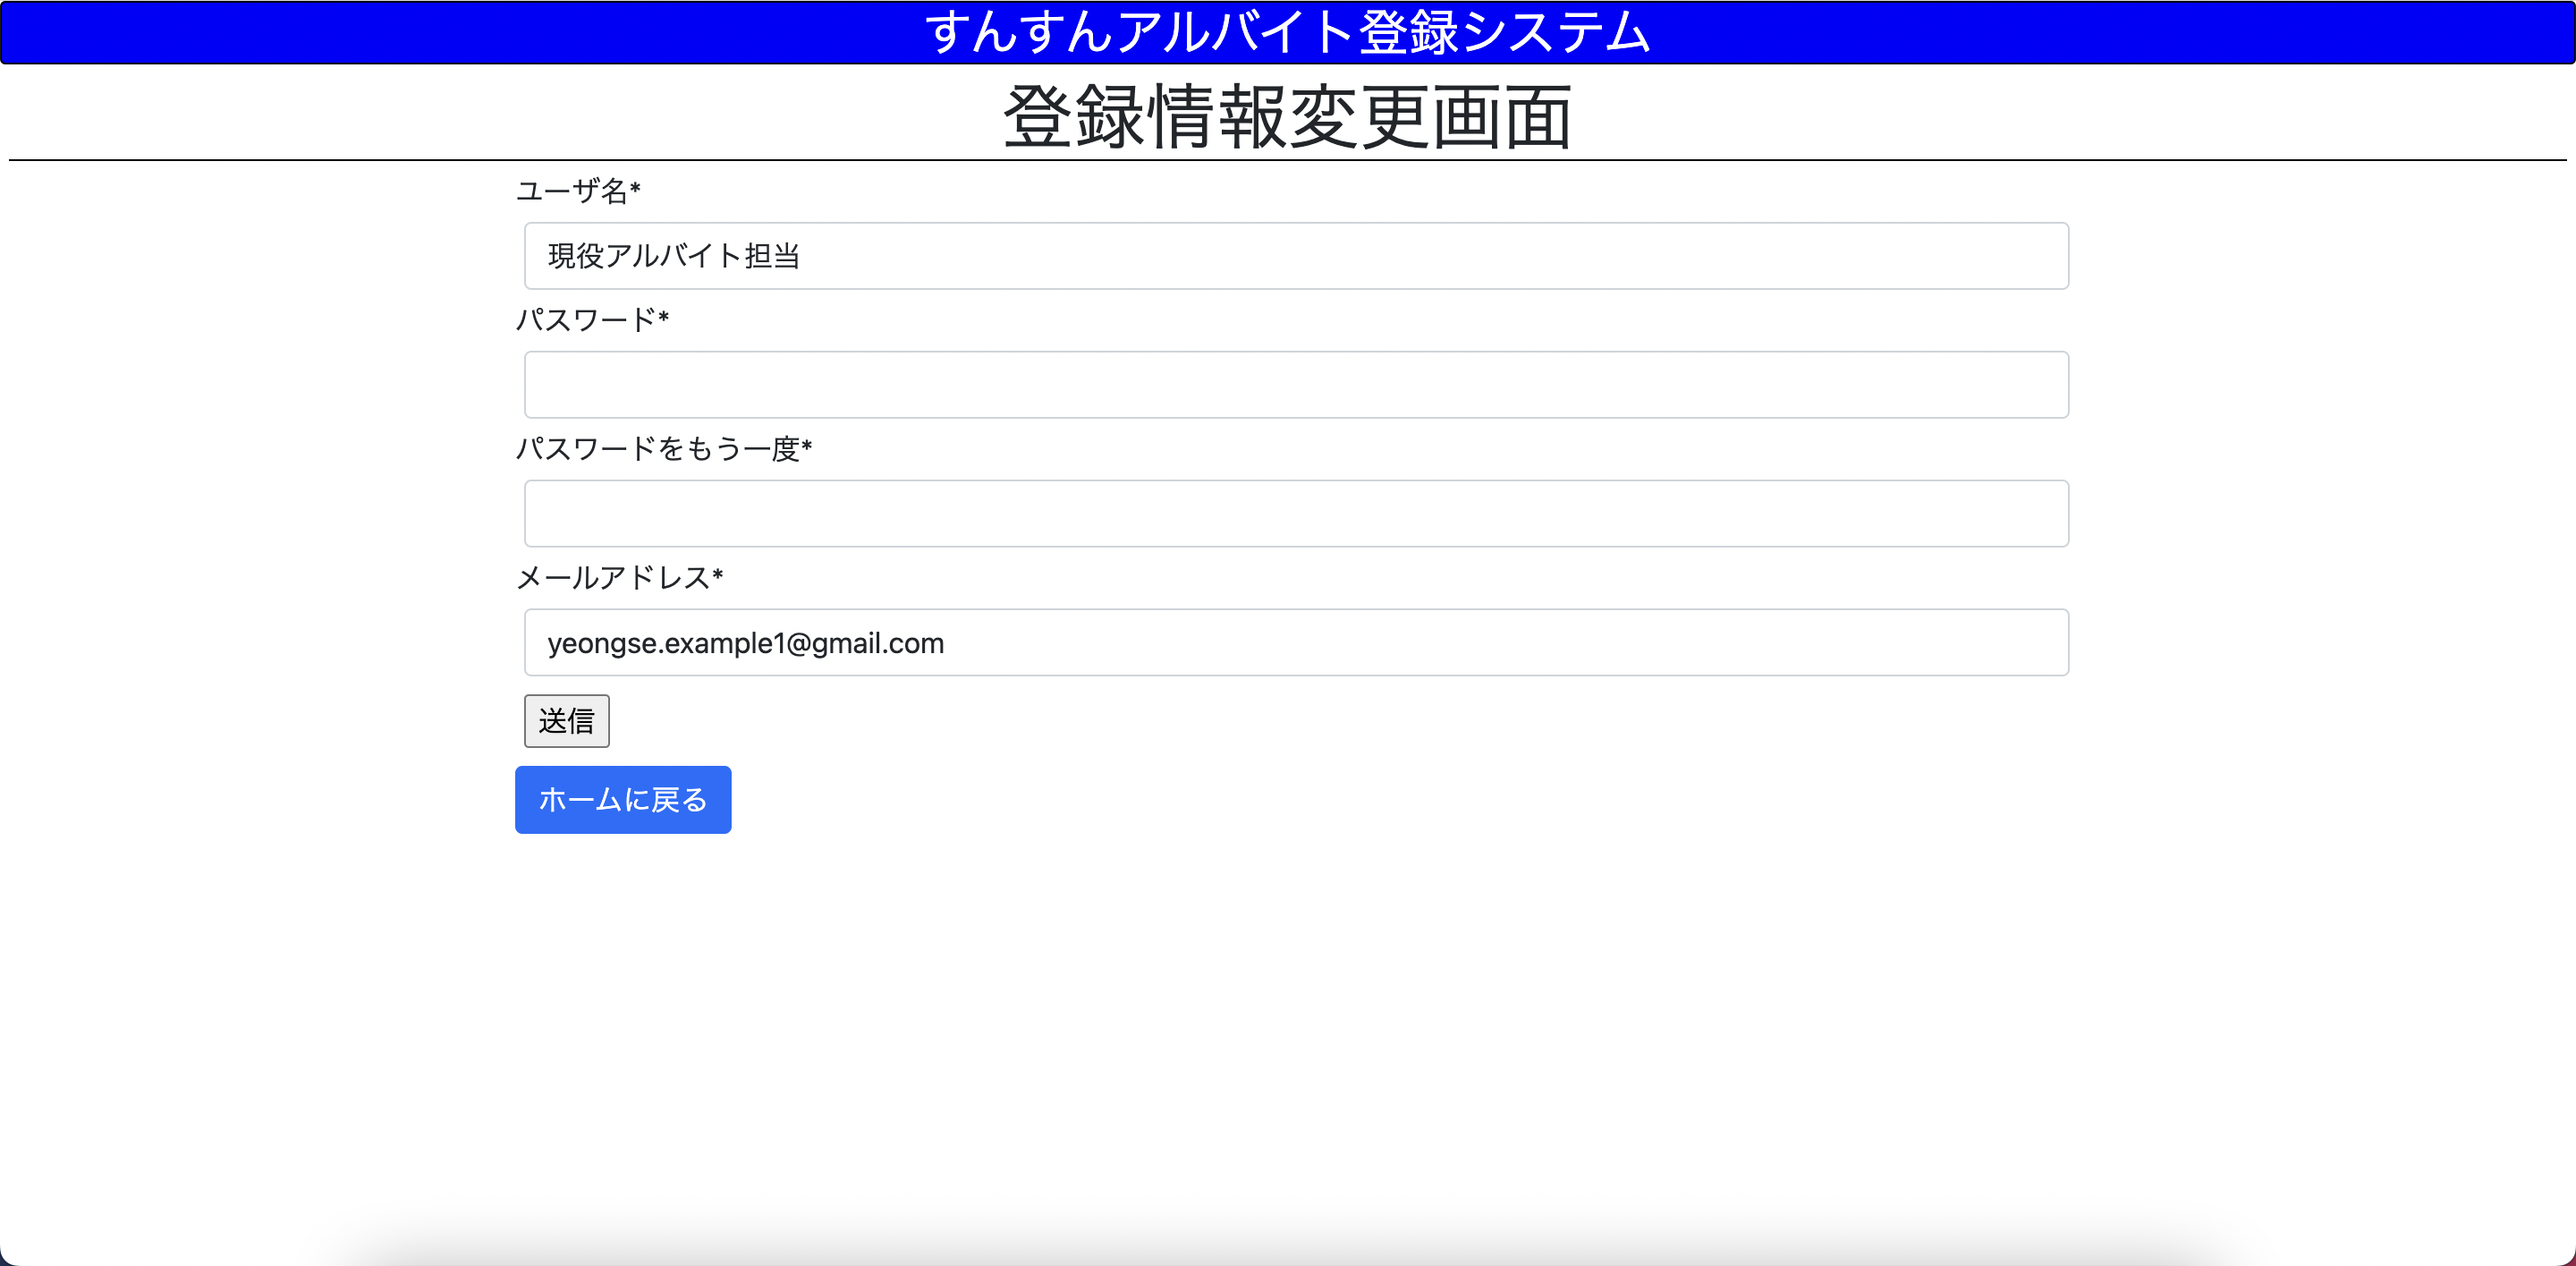
\includegraphics[width=0.8\linewidth]{../figure/9_personal.png}
					}
		\end{figure}
		この画面では登録されている情報(名前、パスワード、メールアドレス)の変更を行うことができます。
		名前とメールアドレスについては、現在登録されている値がデフォルトで入っています。
		変更したい場合はこれを書き換えてください。
		パスワードについては古いものを入力する必要はなく、新しく登録したいものを二回入力します。

	\subsection{開発者へのフィードバック画面}
		\begin{figure}[htbp]
			\centering
			\fbox{
					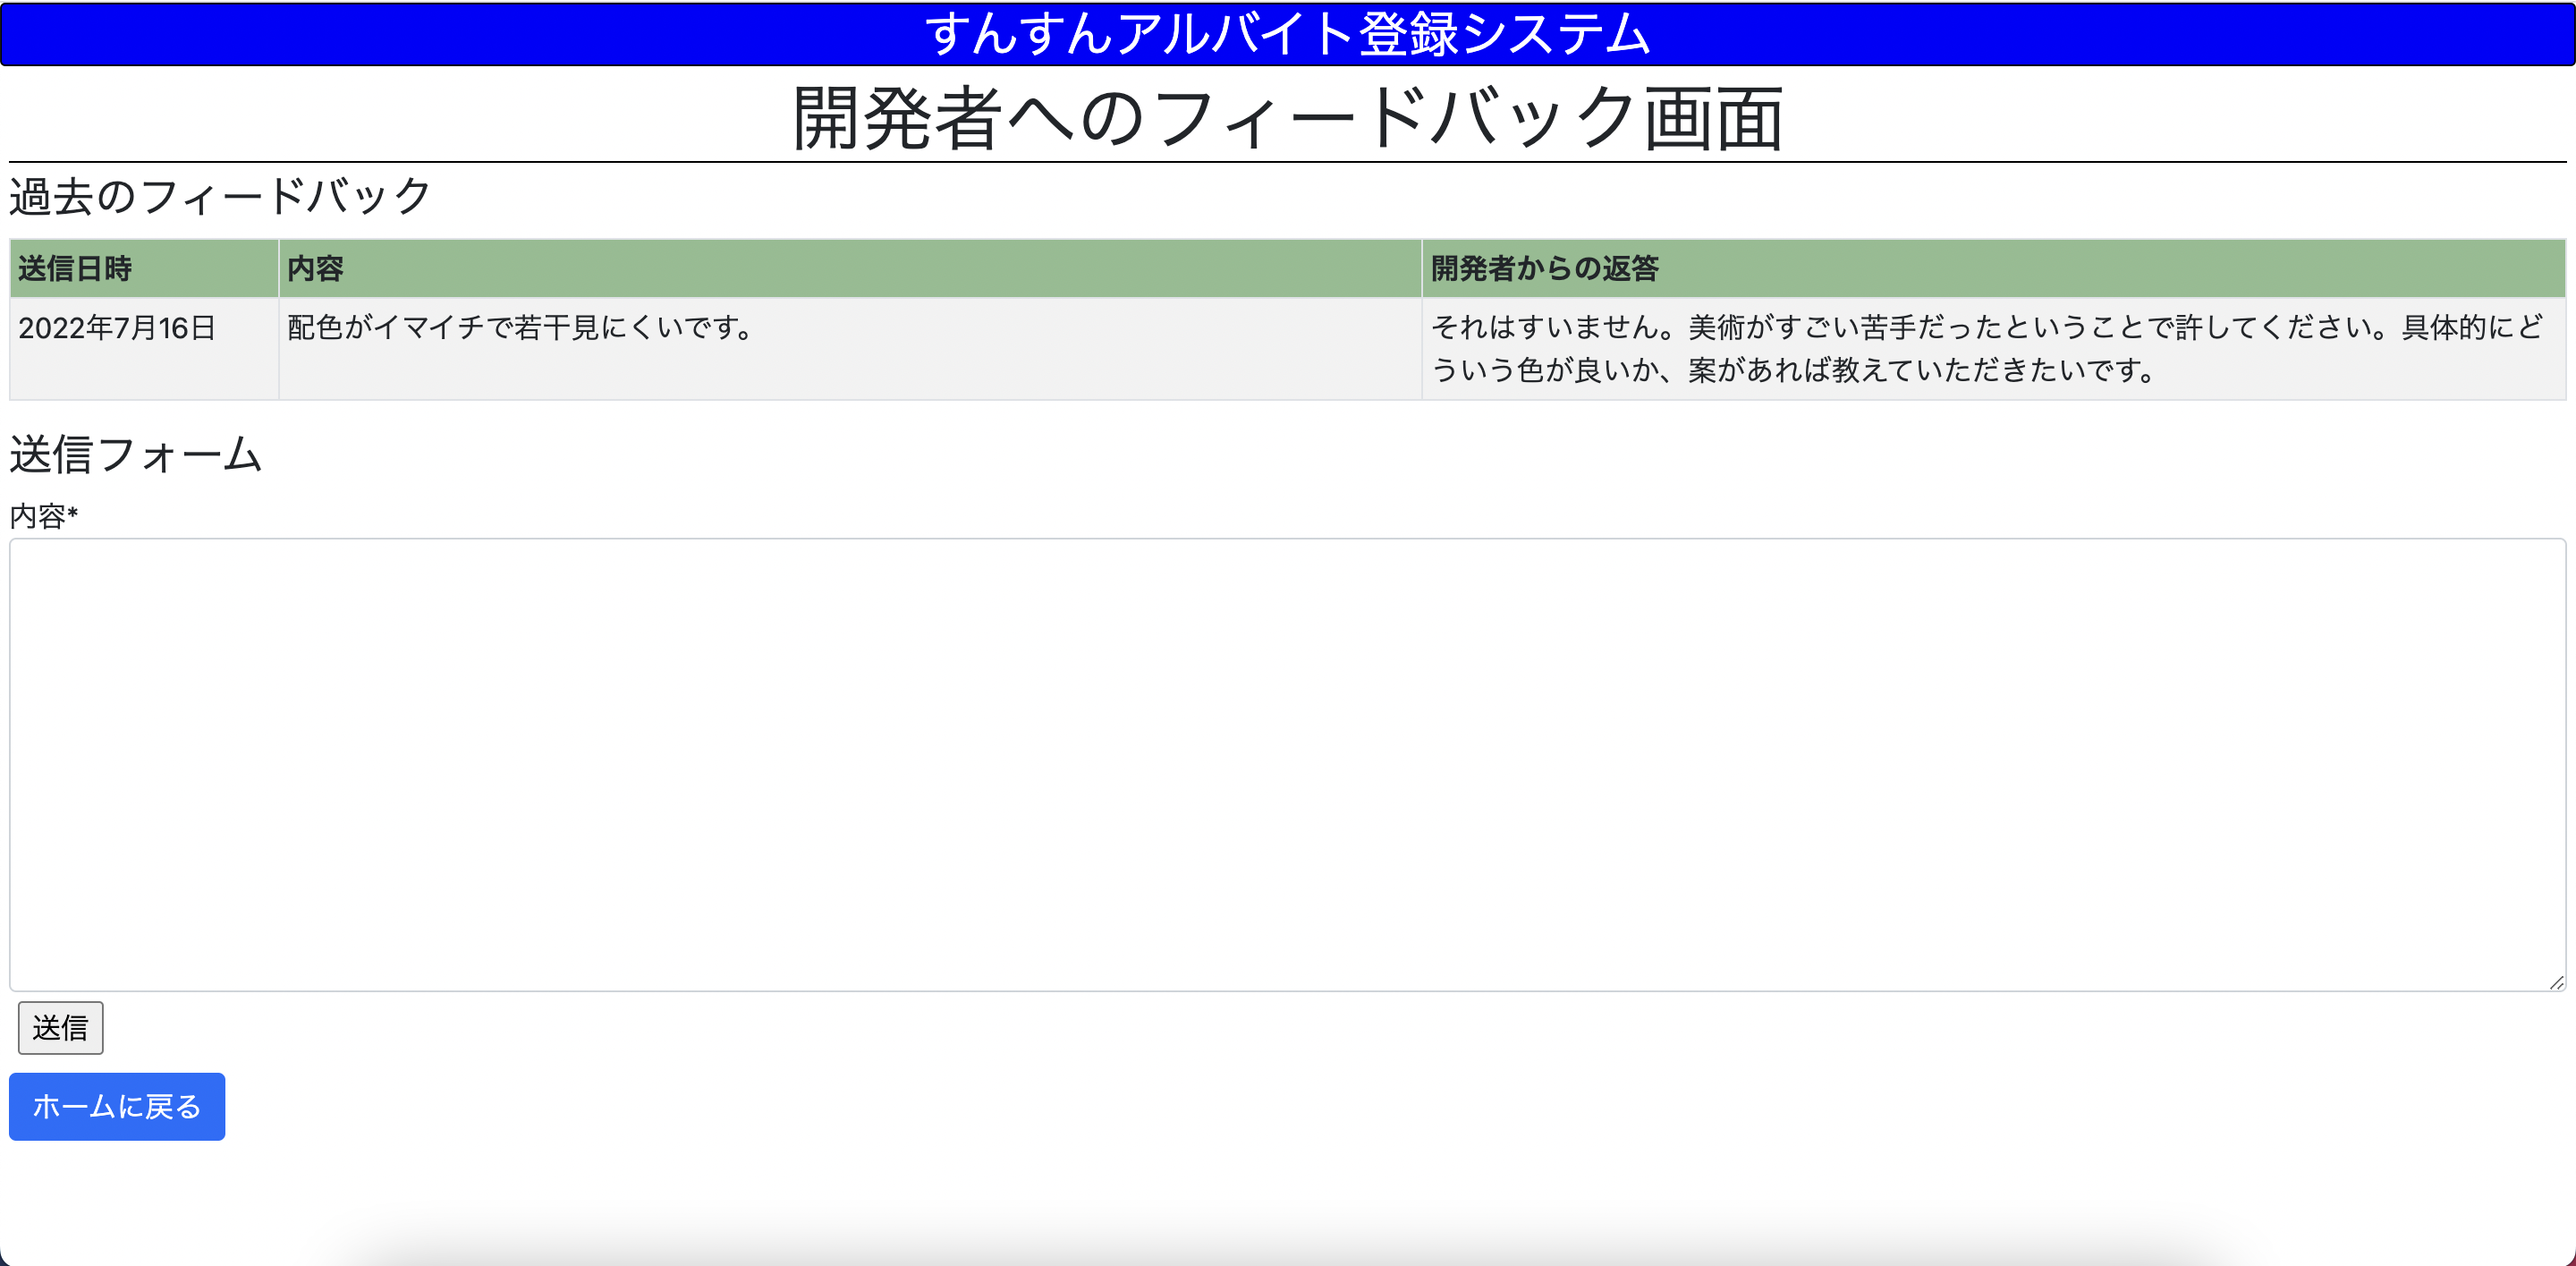
\includegraphics[width=0.8\linewidth]{../figure/10_feedback.png}
				}
		\end{figure}
		この画面では開発者(金栄世)に対してフィードバックを送信することができます。
		送信されたフィードバックについては、後日開発者からの回答が掲載されますので気長にお待ちください。


\section{社員の操作方法}
	\subsection{ホーム画面}
		\begin{figure}[htbp]
			\centering
			\fbox{
					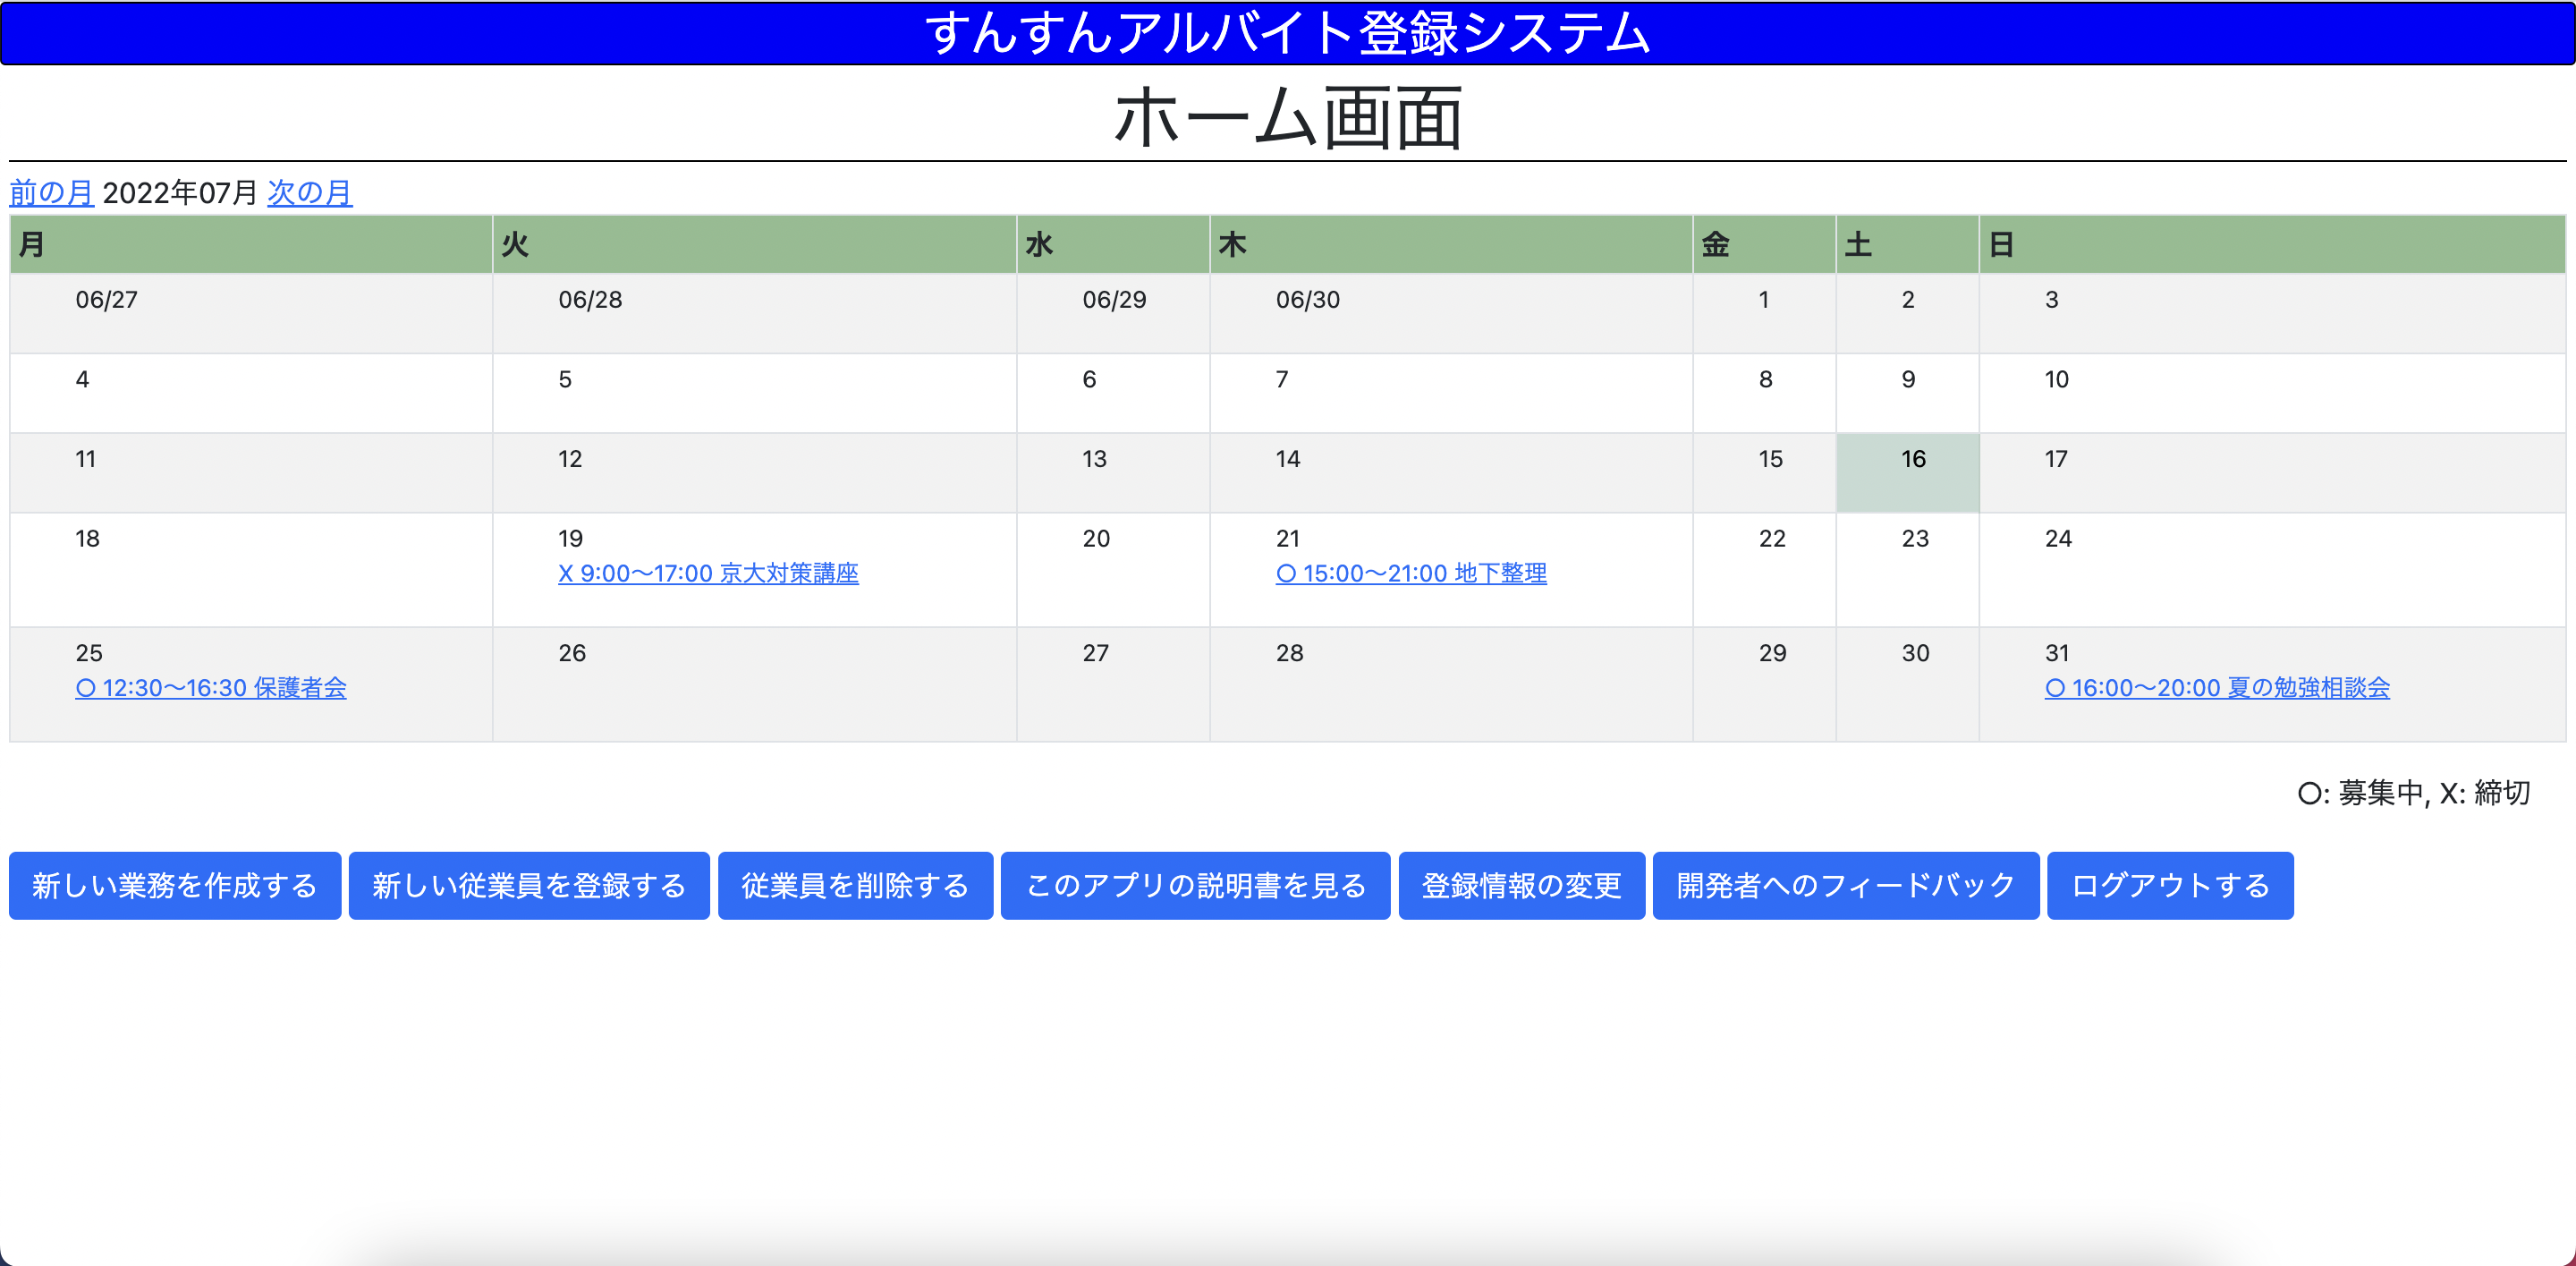
\includegraphics[width=0.8\linewidth]{../figure/2_home_admin.png}
				}
		\end{figure}
		こちらが社員用のホーム画面になります。
		ホーム画面はカレンダーと様々なページへ遷移するためのボタンで構成されています。
		何かしらこのアプリケーションで作業を行った場合、このホーム画面へと遷移するように構成されています。
		\par

		デフォルトでは今の月のカレンダーが表示されますが、カレンダー上部の「前の月」と「次の月」をクリックすることで他の月のカレンダーを表示させることができます。
		カレンダー内にはその月に募集している業務が表示されます。
		先頭に丸印がついているものは現在募集中のもの、バツ印がついているものは募集を締め切ったものを表しています。
		カレンダー内の業務をクリックすると、その業務の詳細画面へと移動できます(2.2を参照)。
		\par

		カレンダーの下のボタンを押すと、それぞれ別の画面へと遷移します(2.3〜2.8を参照)。
		また、ホーム画面からログアウトすることができます。
		\clearpage


	\subsection{業務詳細画面}
		\begin{figure}[htbp]
			\centering
			\fbox{
					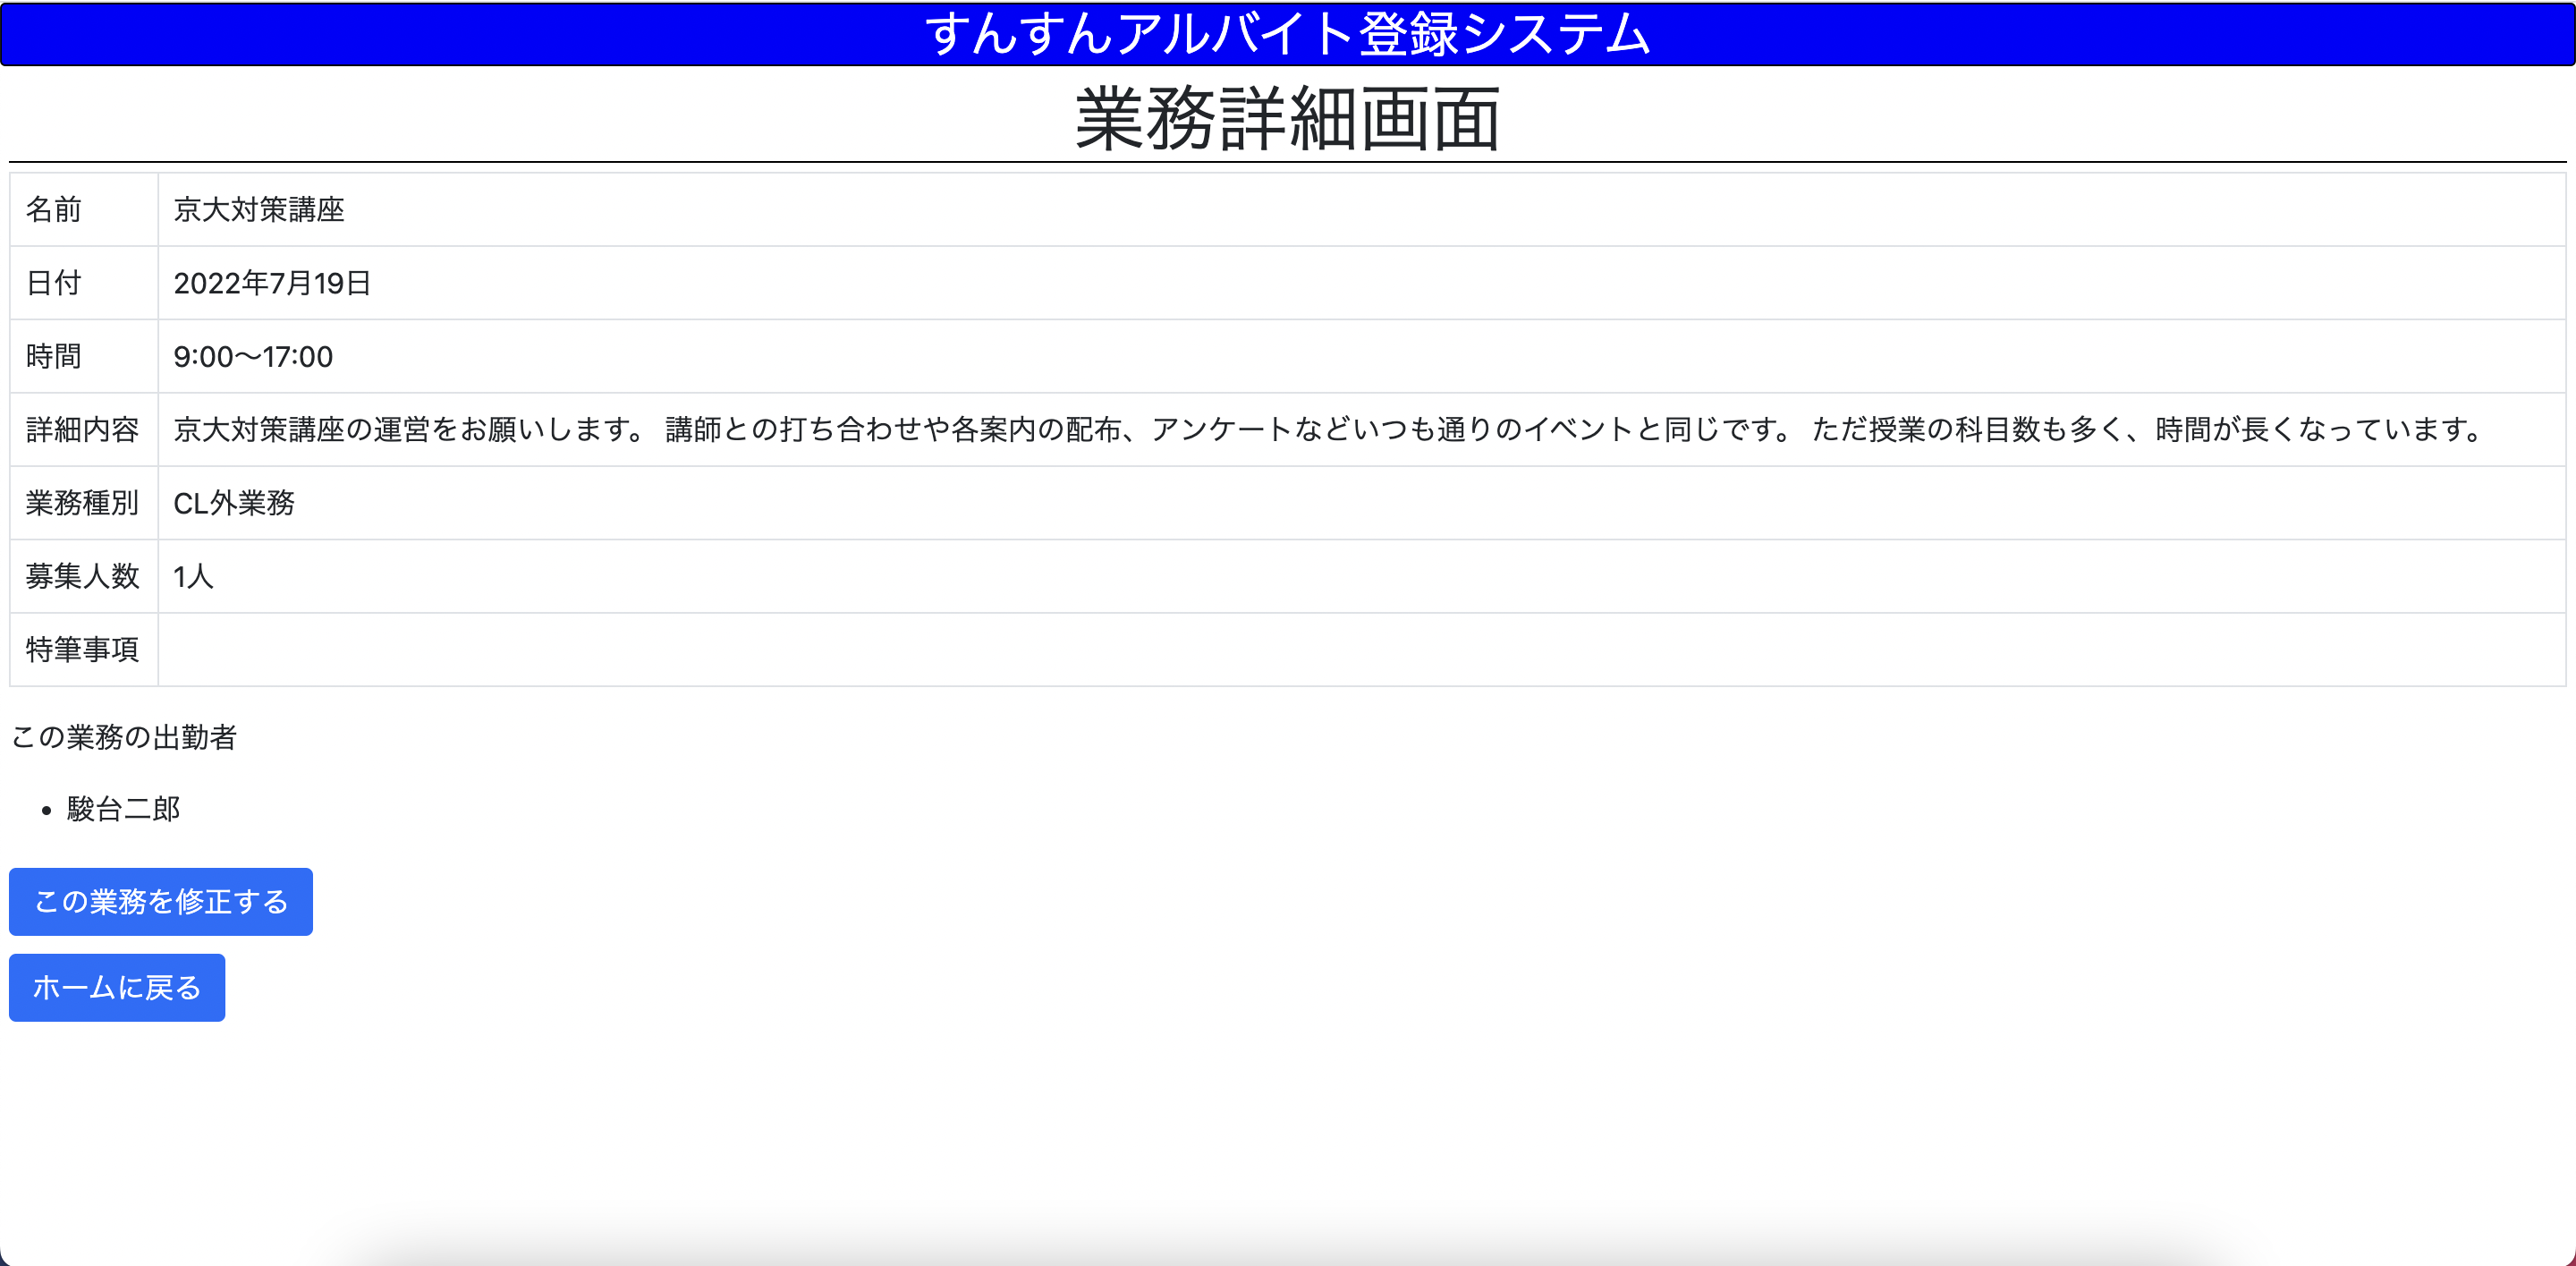
\includegraphics[width=0.8\linewidth]{../figure/3_specification_admin.png}
				}
		\end{figure}
		こちらが業務詳細画面になります。
		この画面では業務の詳細内容を確認することができます。
		表の下部には現在応募済みの従業員の名前が掲載されています。
		また、最下部のボタンからこの業務の修正画面に遷移することができます(2.3を参照)。
		\clearpage


	\subsection{業務修正画面}
		\begin{figure}[htbp]
			\begin{minipage}[b]{\linewidth}
				\centering
				\fbox{
					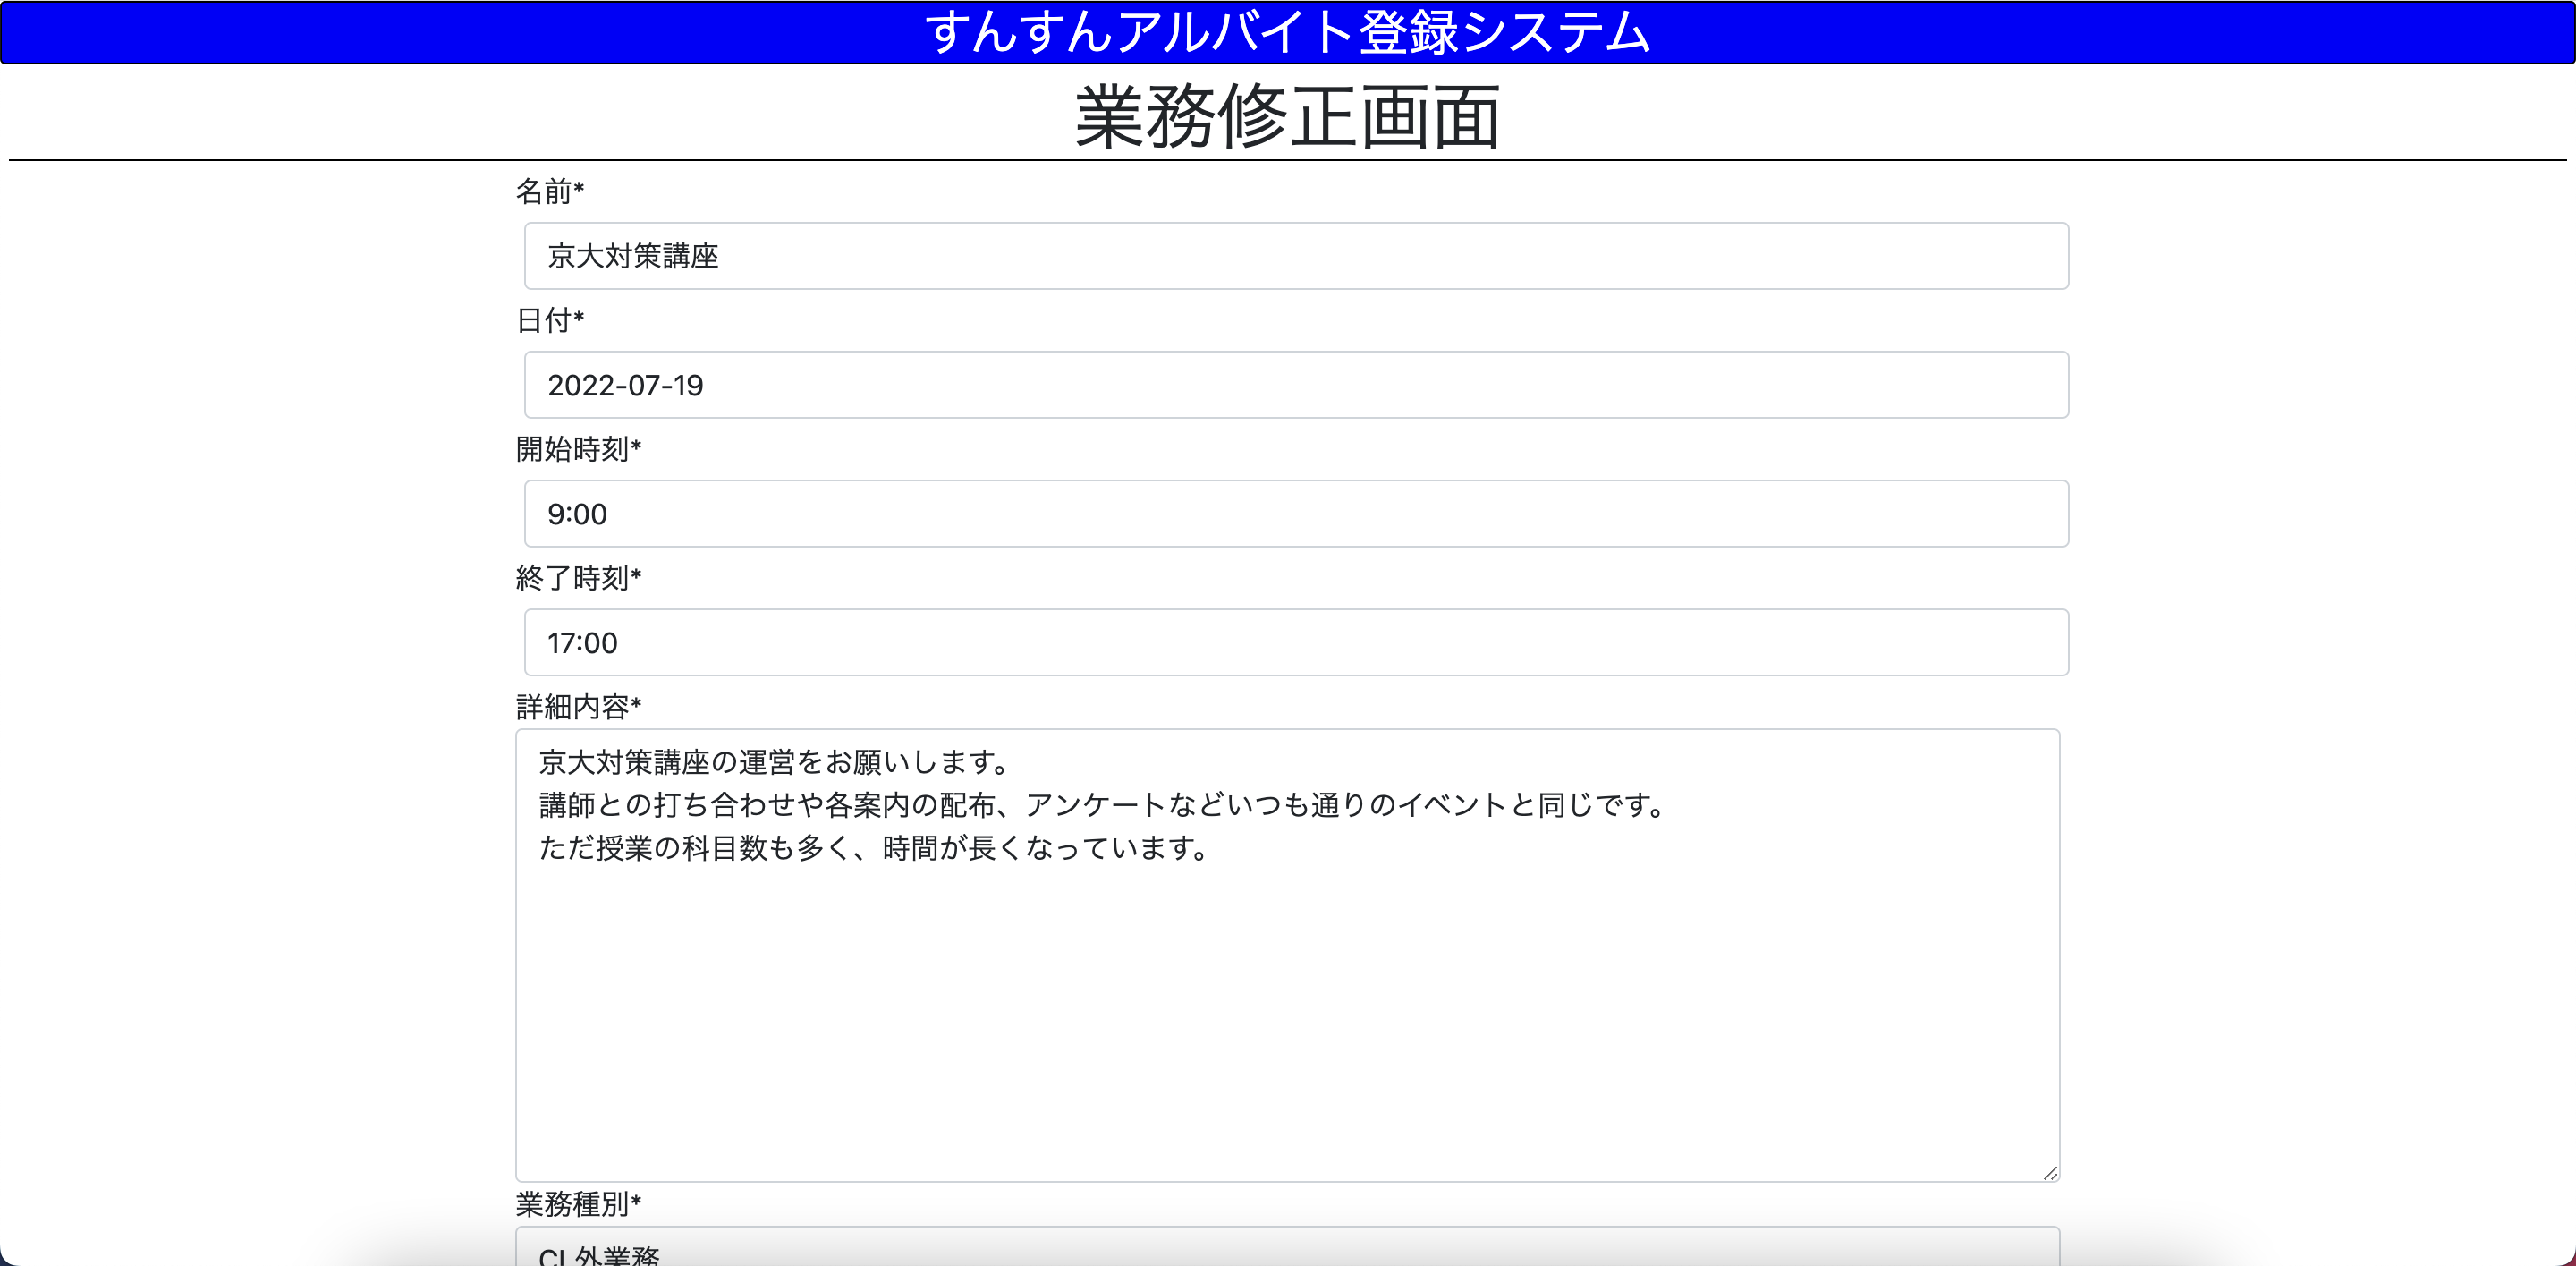
\includegraphics[width=0.8\linewidth]{../figure/4_revise_1.png}
				}
			\end{minipage} \\
			\begin{minipage}[b]{\linewidth}
				\centering
				\fbox{
					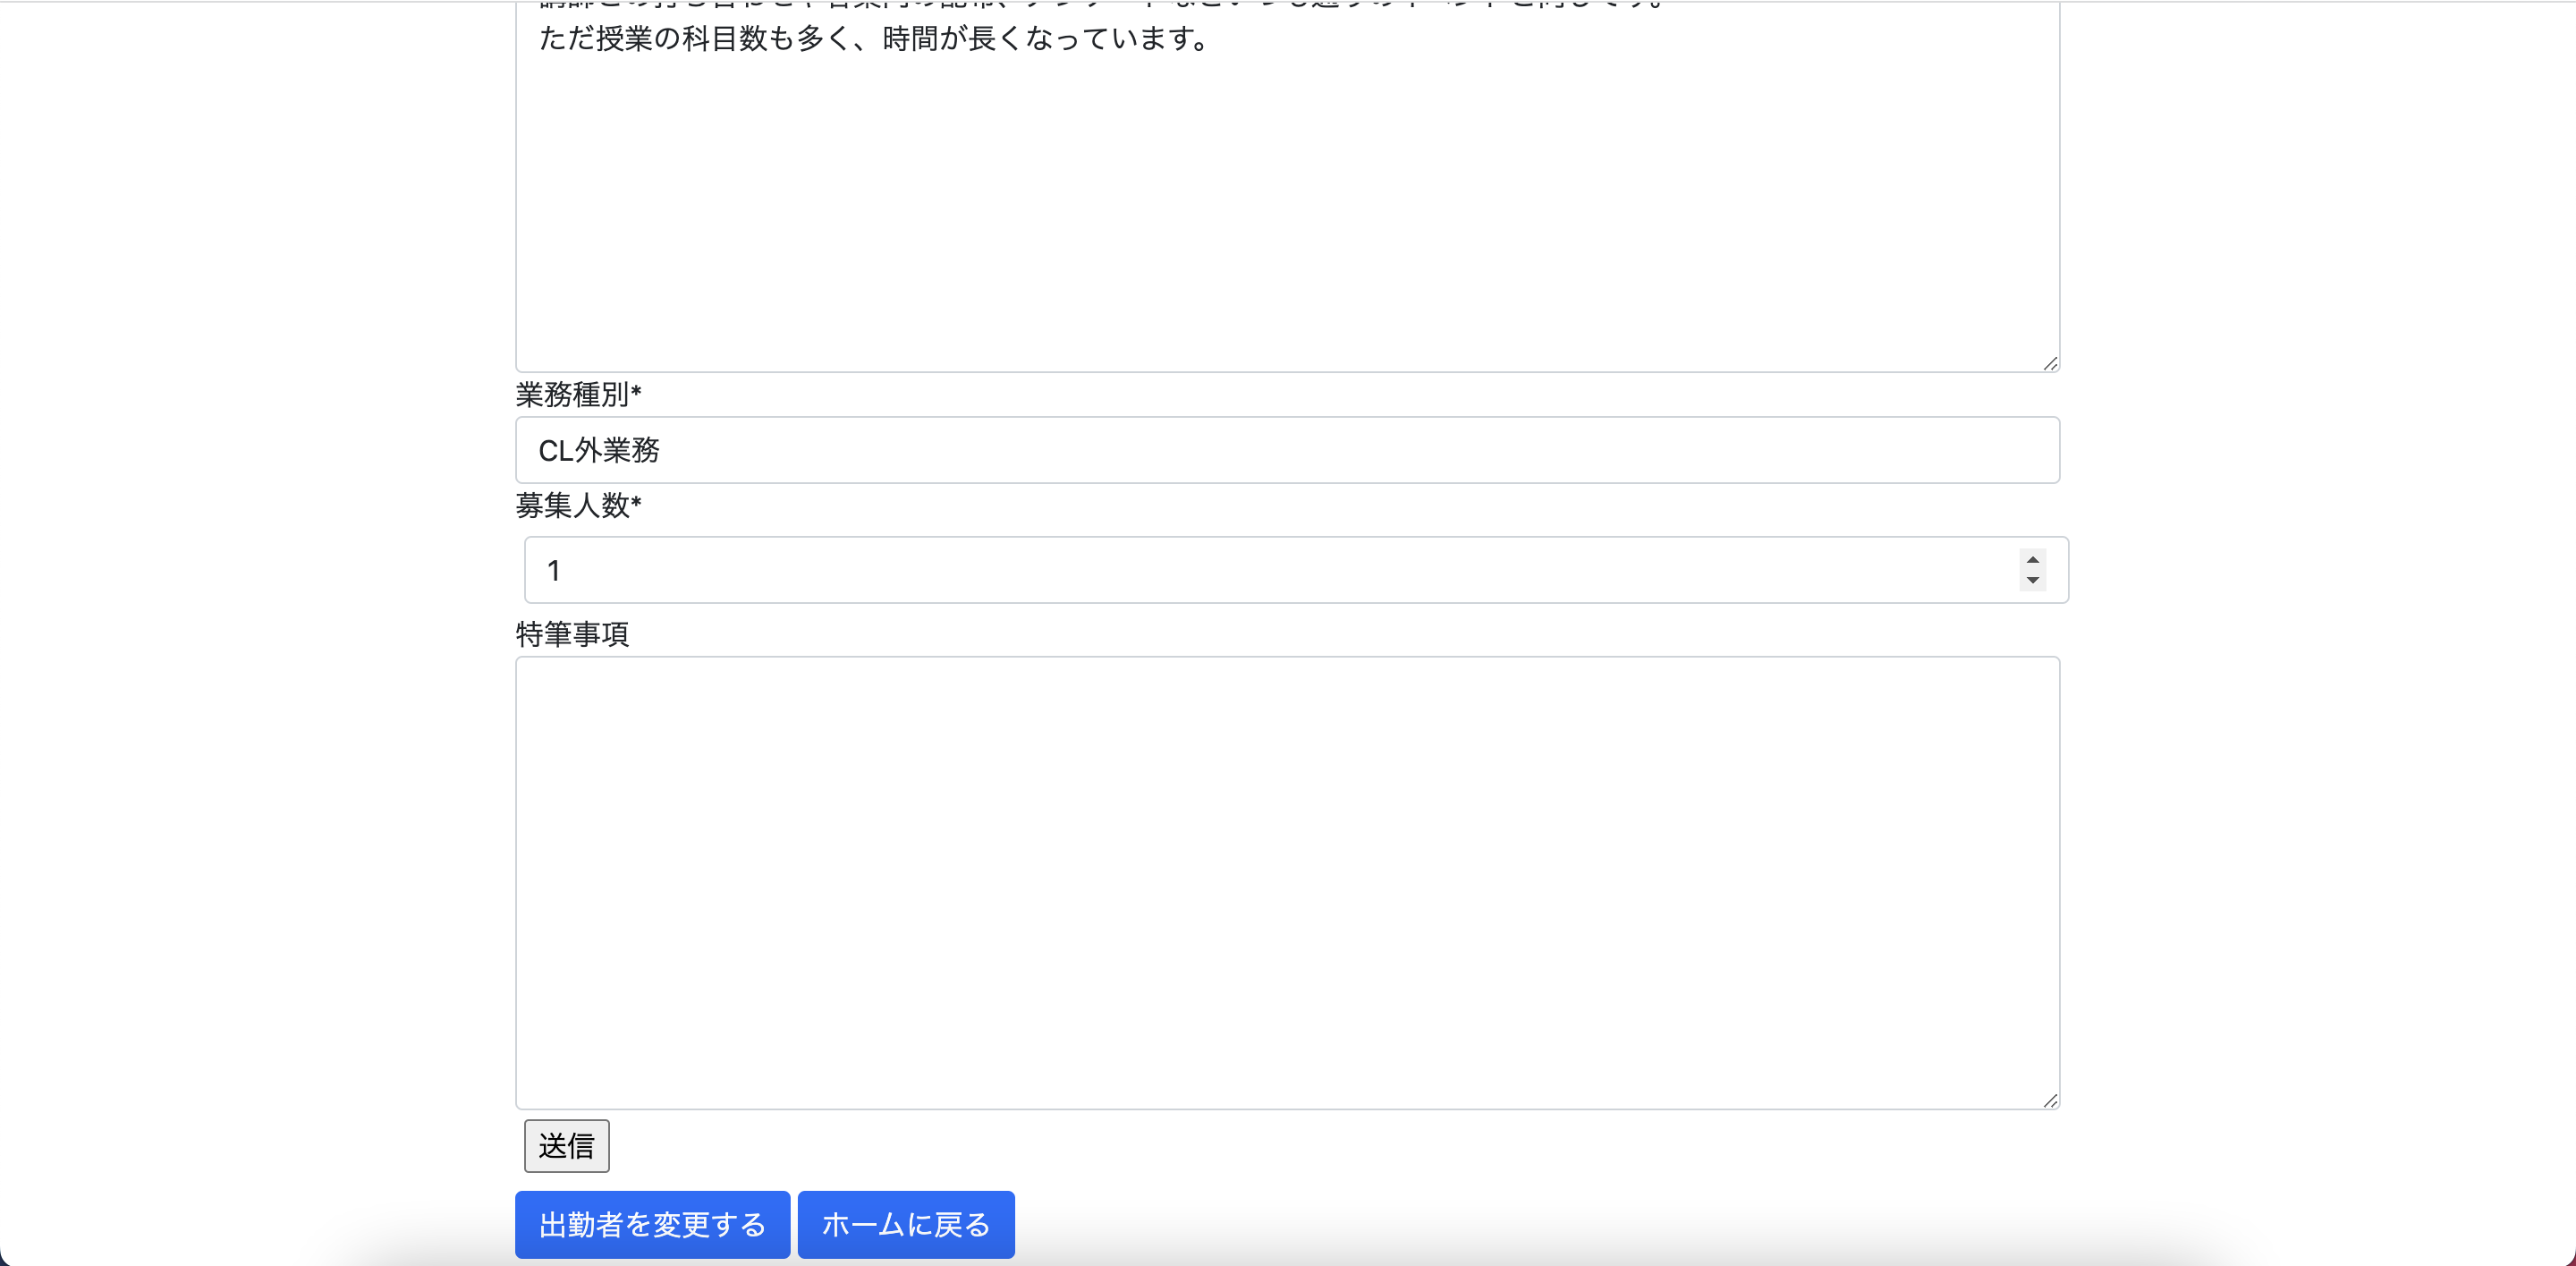
\includegraphics[width=0.8\linewidth]{../figure/4_revise_2.png}
				}
			\end{minipage}
		\end{figure}
		こちらが業務修正画面になります。
		作成済みの業務について、各項目を自由に変更することができます。
		また最下部のボタンから出勤者を変更することができます。
		\clearpage


	\subsection{出勤者変更画面}
		\begin{figure}[htbp]
			\centering
			\fbox{
					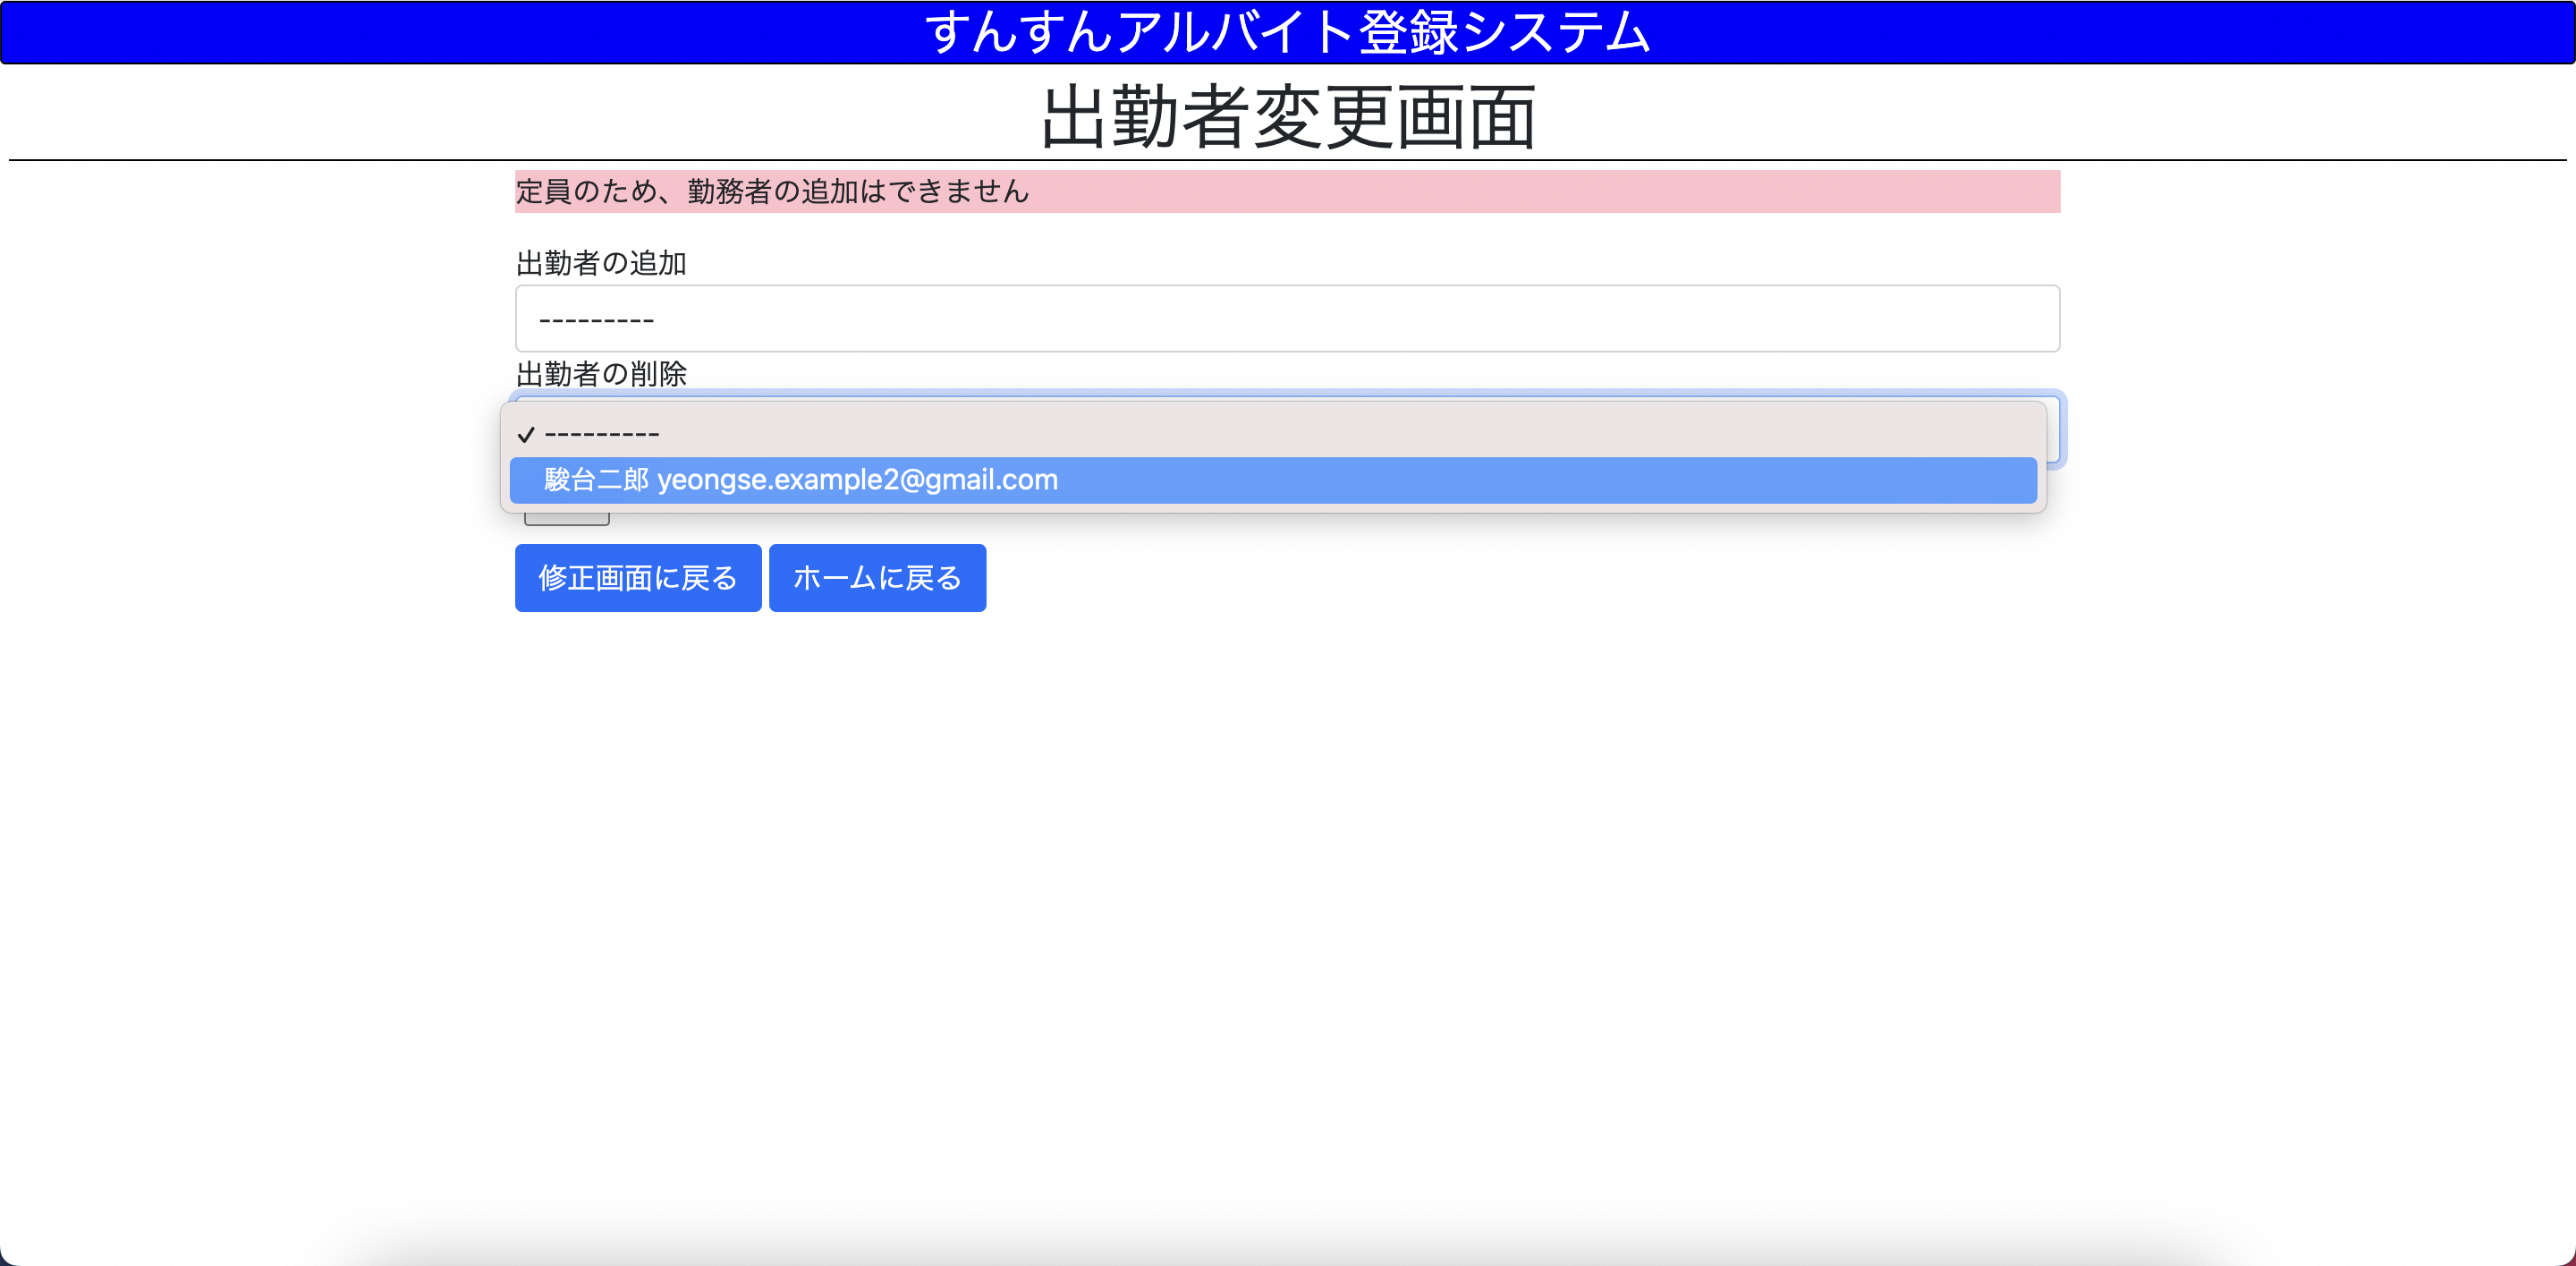
\includegraphics[width=0.8\linewidth]{../figure/5_reassign.png}
				}
		\end{figure}
		こちらが出勤者変更画面になります。
		やむを得ず出勤ができなくなった場合や、社員が直接出勤者の追加を行いたい場合に利用してください。
		出勤者の削除は現在応募済みのアルバイトの中から、出勤者の追加はその業務に未応募のアルバイトの中から1人ずつ選択することができます。
		出勤者の数が募集人員に達している場合、図のように出勤者を追加することができなくなります。


	\subsection{新規業務作成画面}
		\begin{figure}[htbp]
			\centering
			\fbox{
					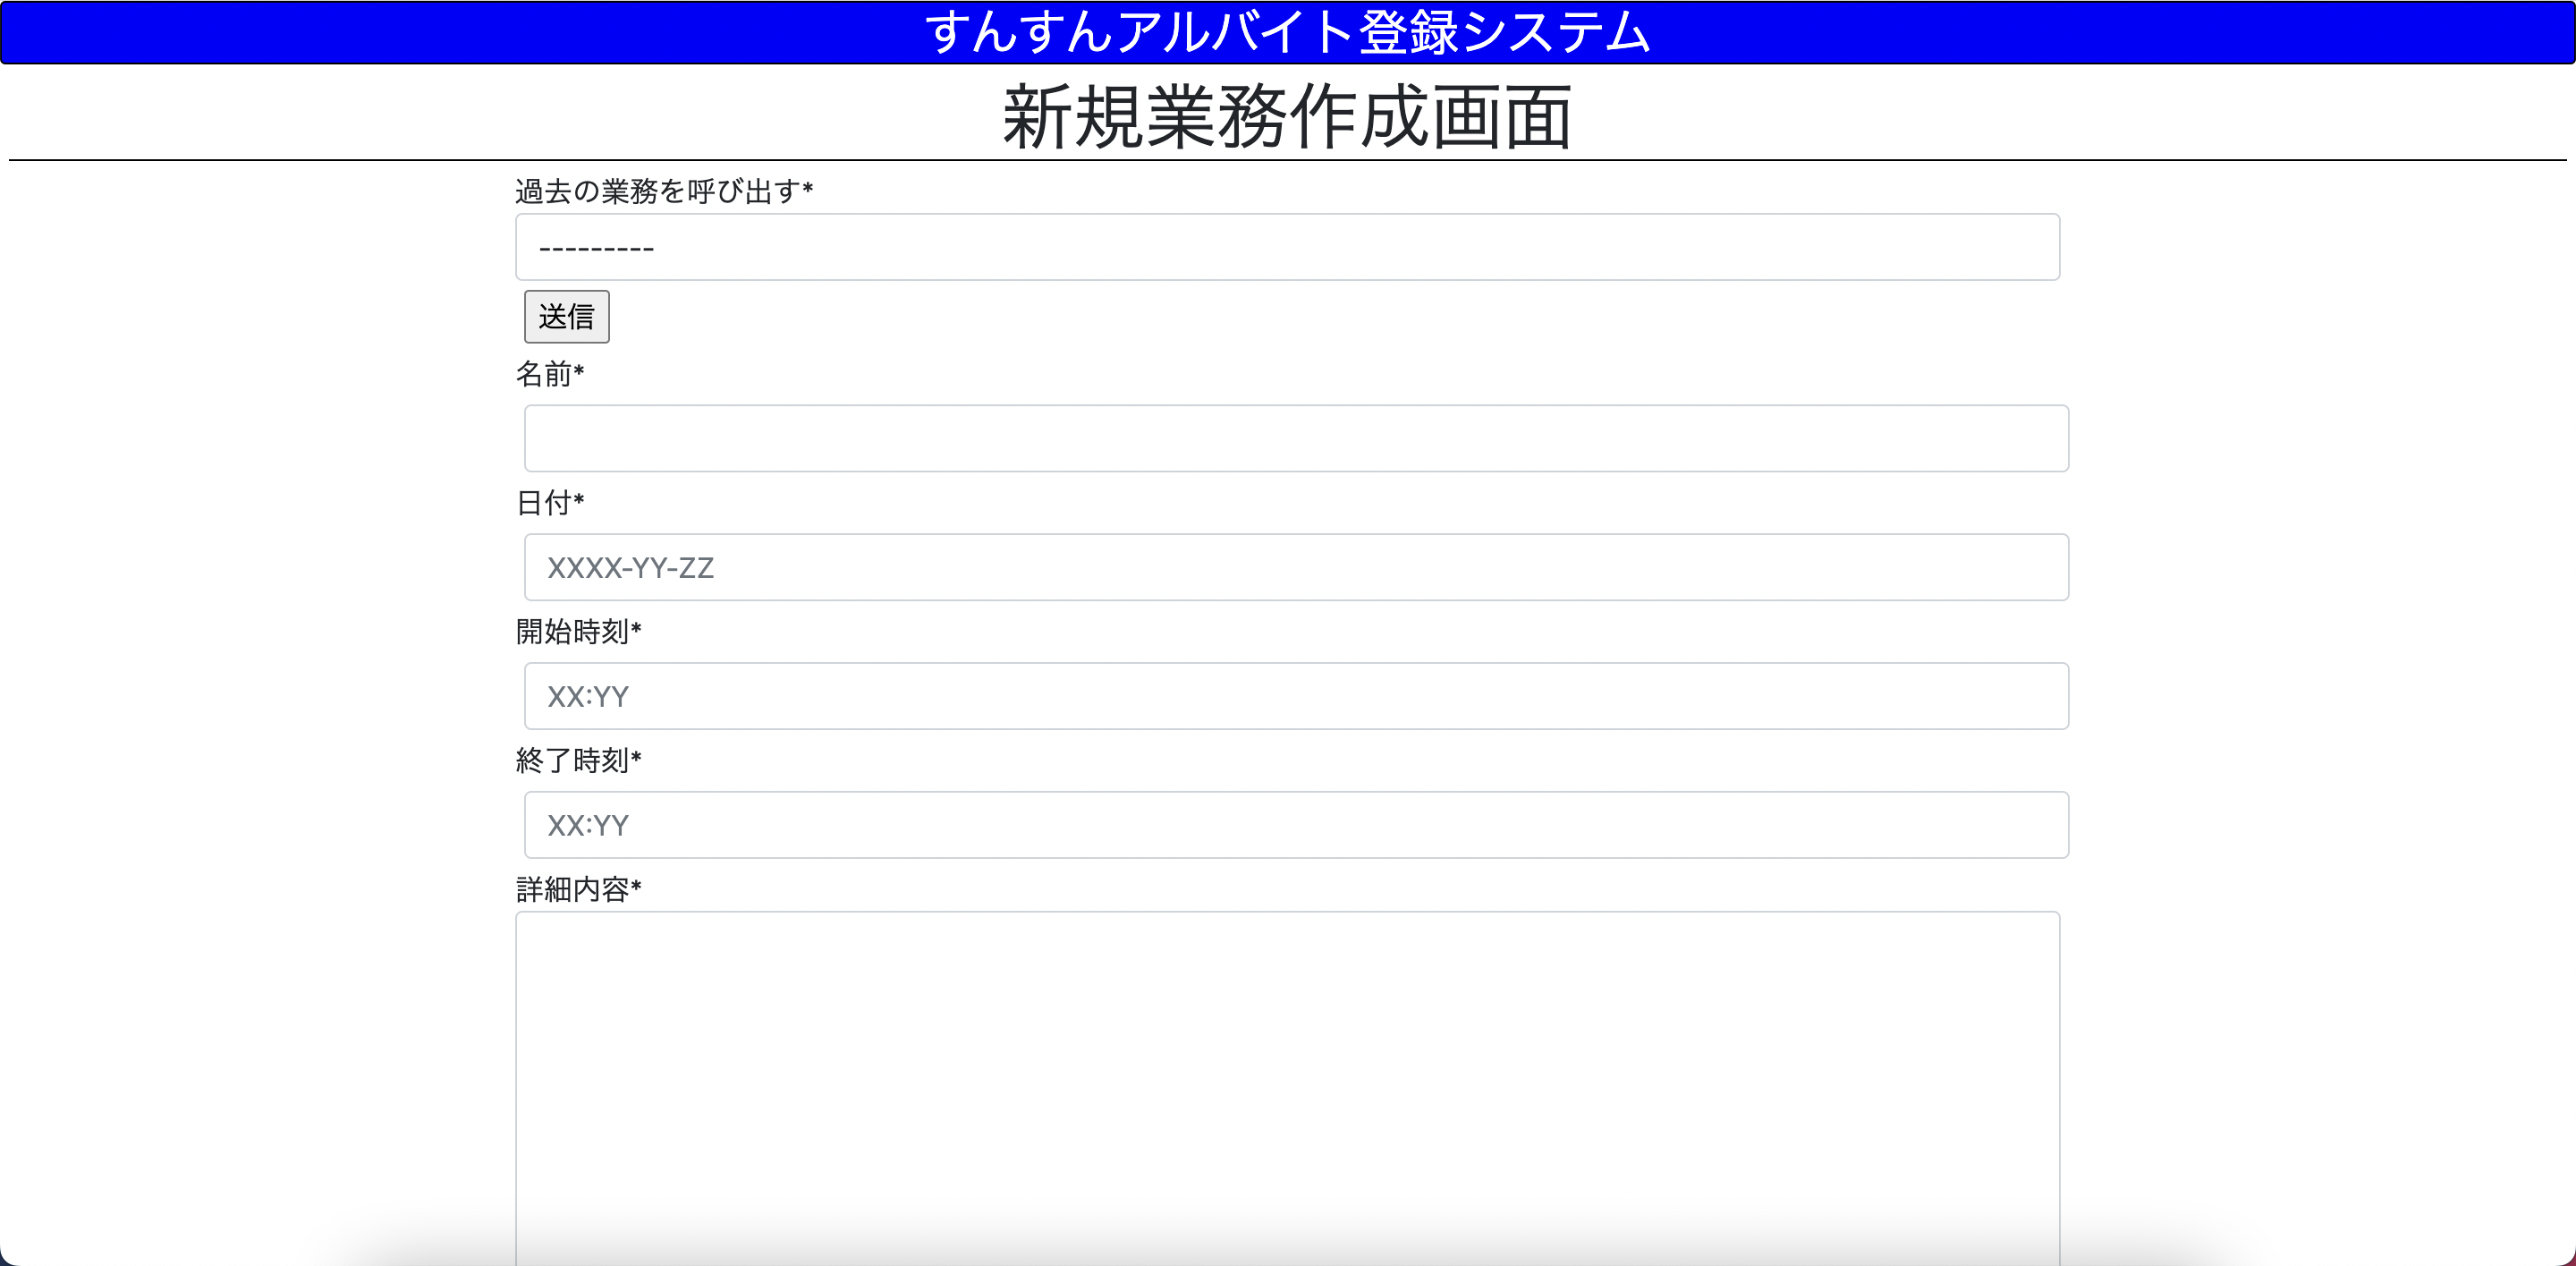
\includegraphics[width=0.8\linewidth]{../figure/6_make_1.png}
				}
		\end{figure}
		こちらが新規業務作成画面になります。
		必要な情報を入力・送信することで業務を作成することができます。
		入力方式が指定されているものについては、指定されている通りに入力してください(日付をXXXX-YY-ZZ、時間をXX:YYなど)。
		\clearpage

		\begin{figure}[htbp]
			\begin{minipage}[b]{\linewidth}
				\centering
				\fbox{
					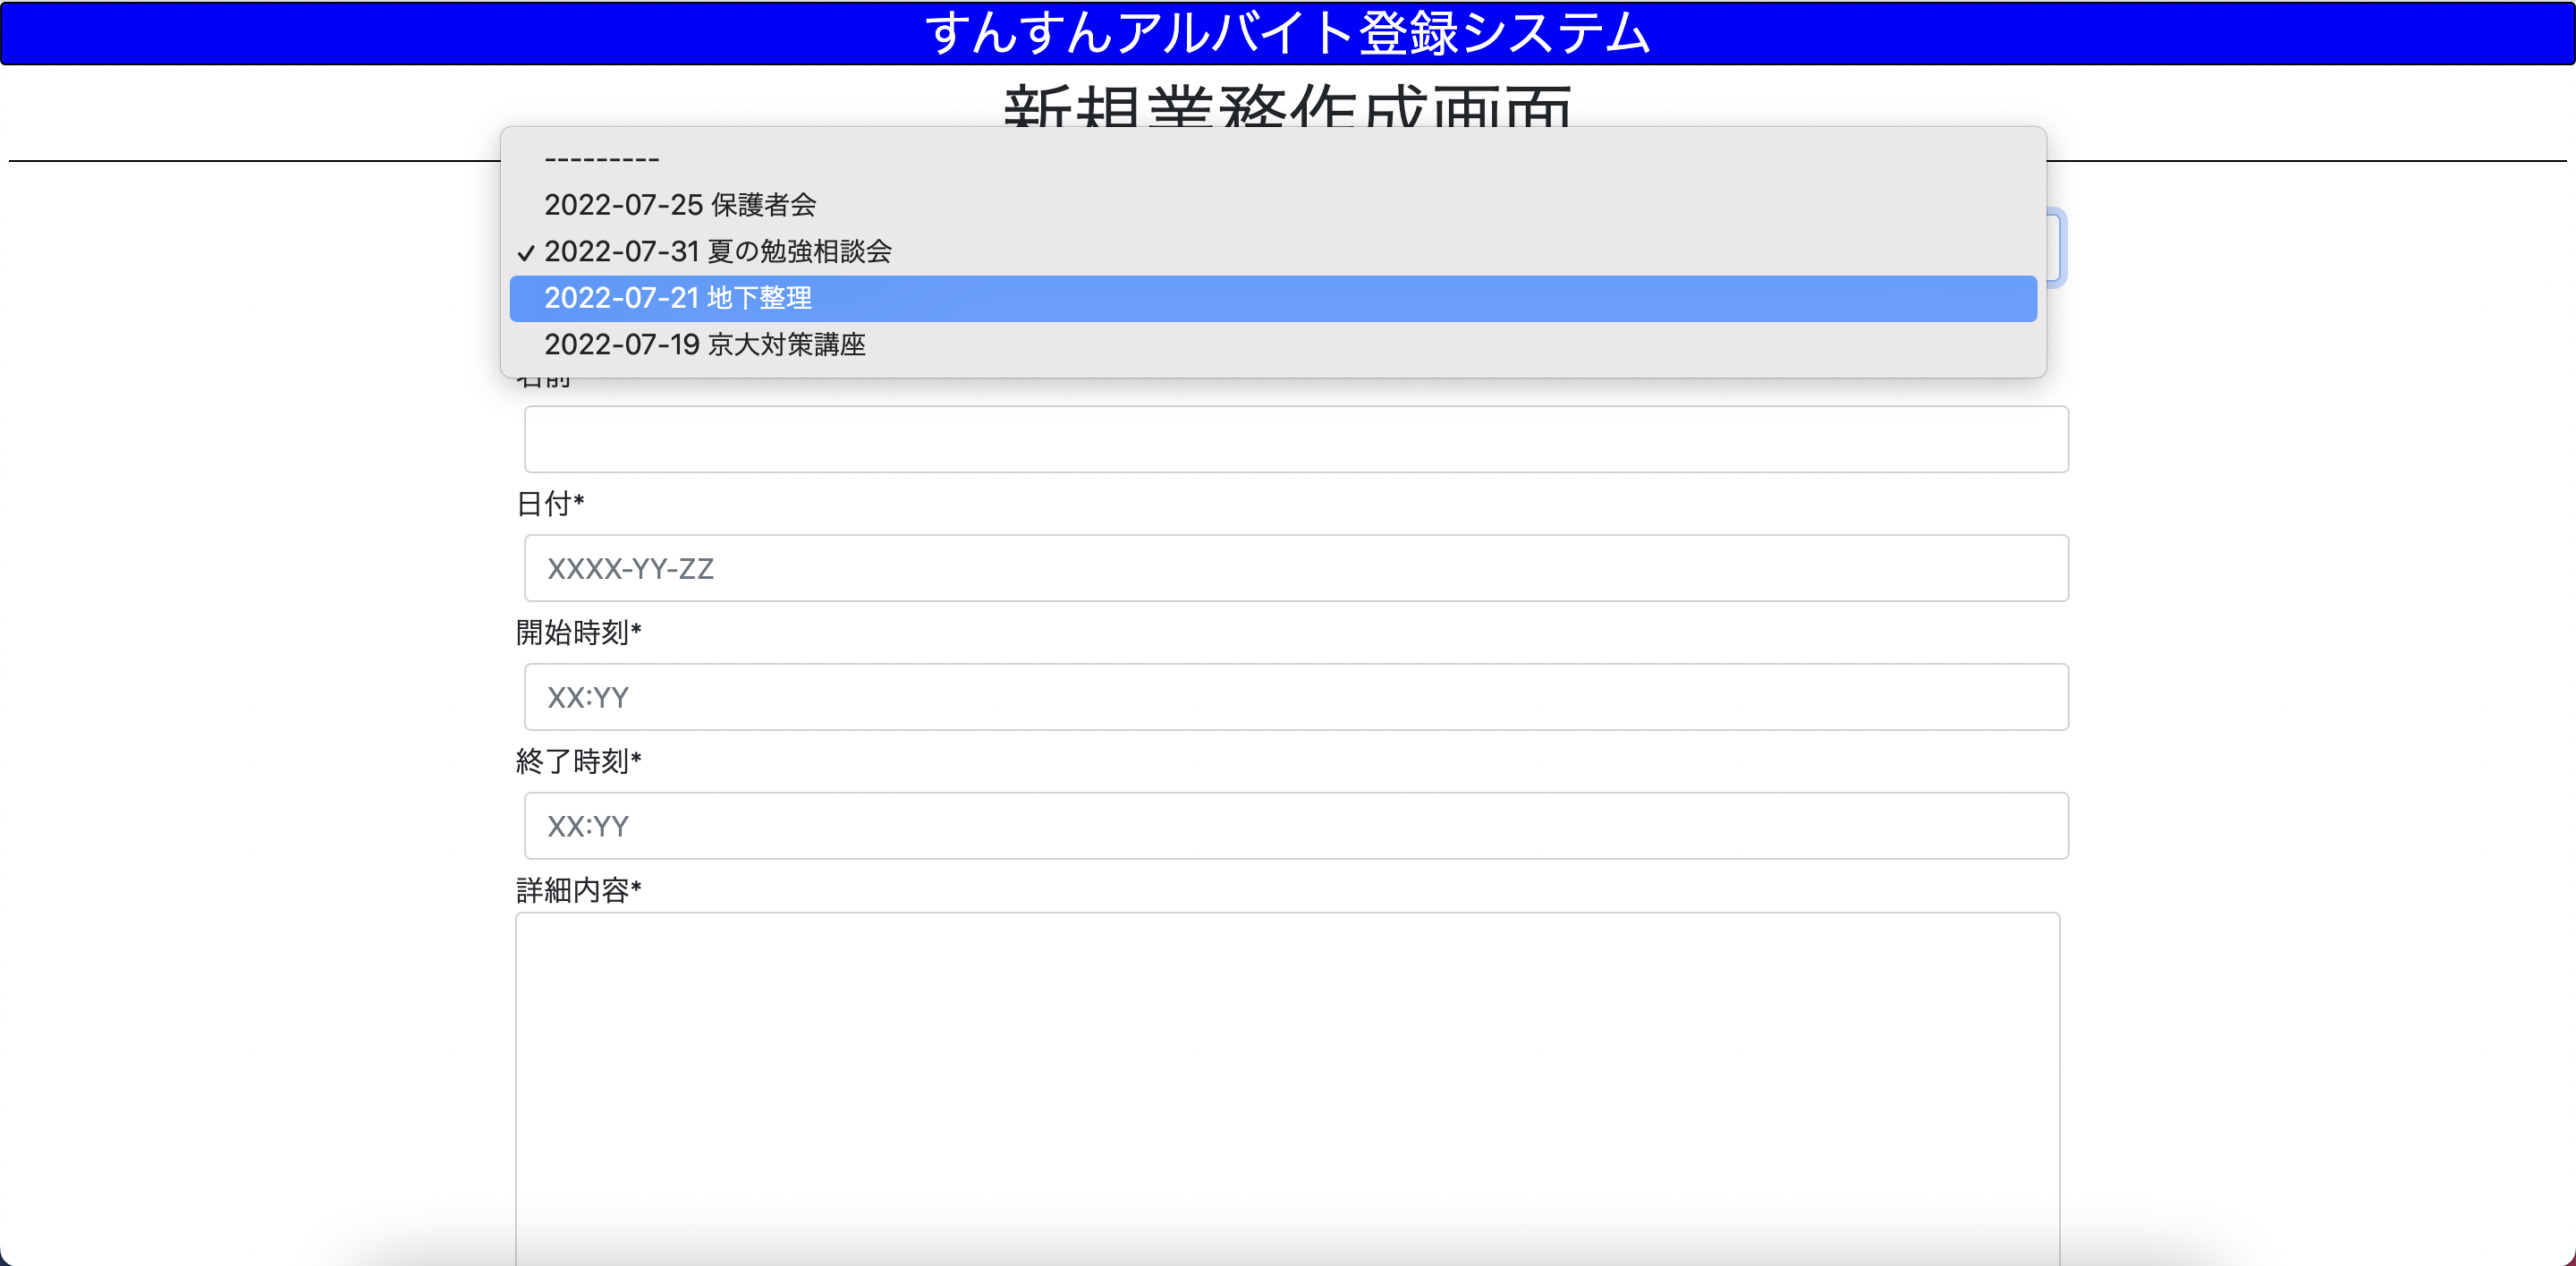
\includegraphics[width=0.8\linewidth]{../figure/6_make_2.png}
				}
			\end{minipage} \\
			\begin{minipage}[b]{\linewidth}
				\centering
				\fbox{
					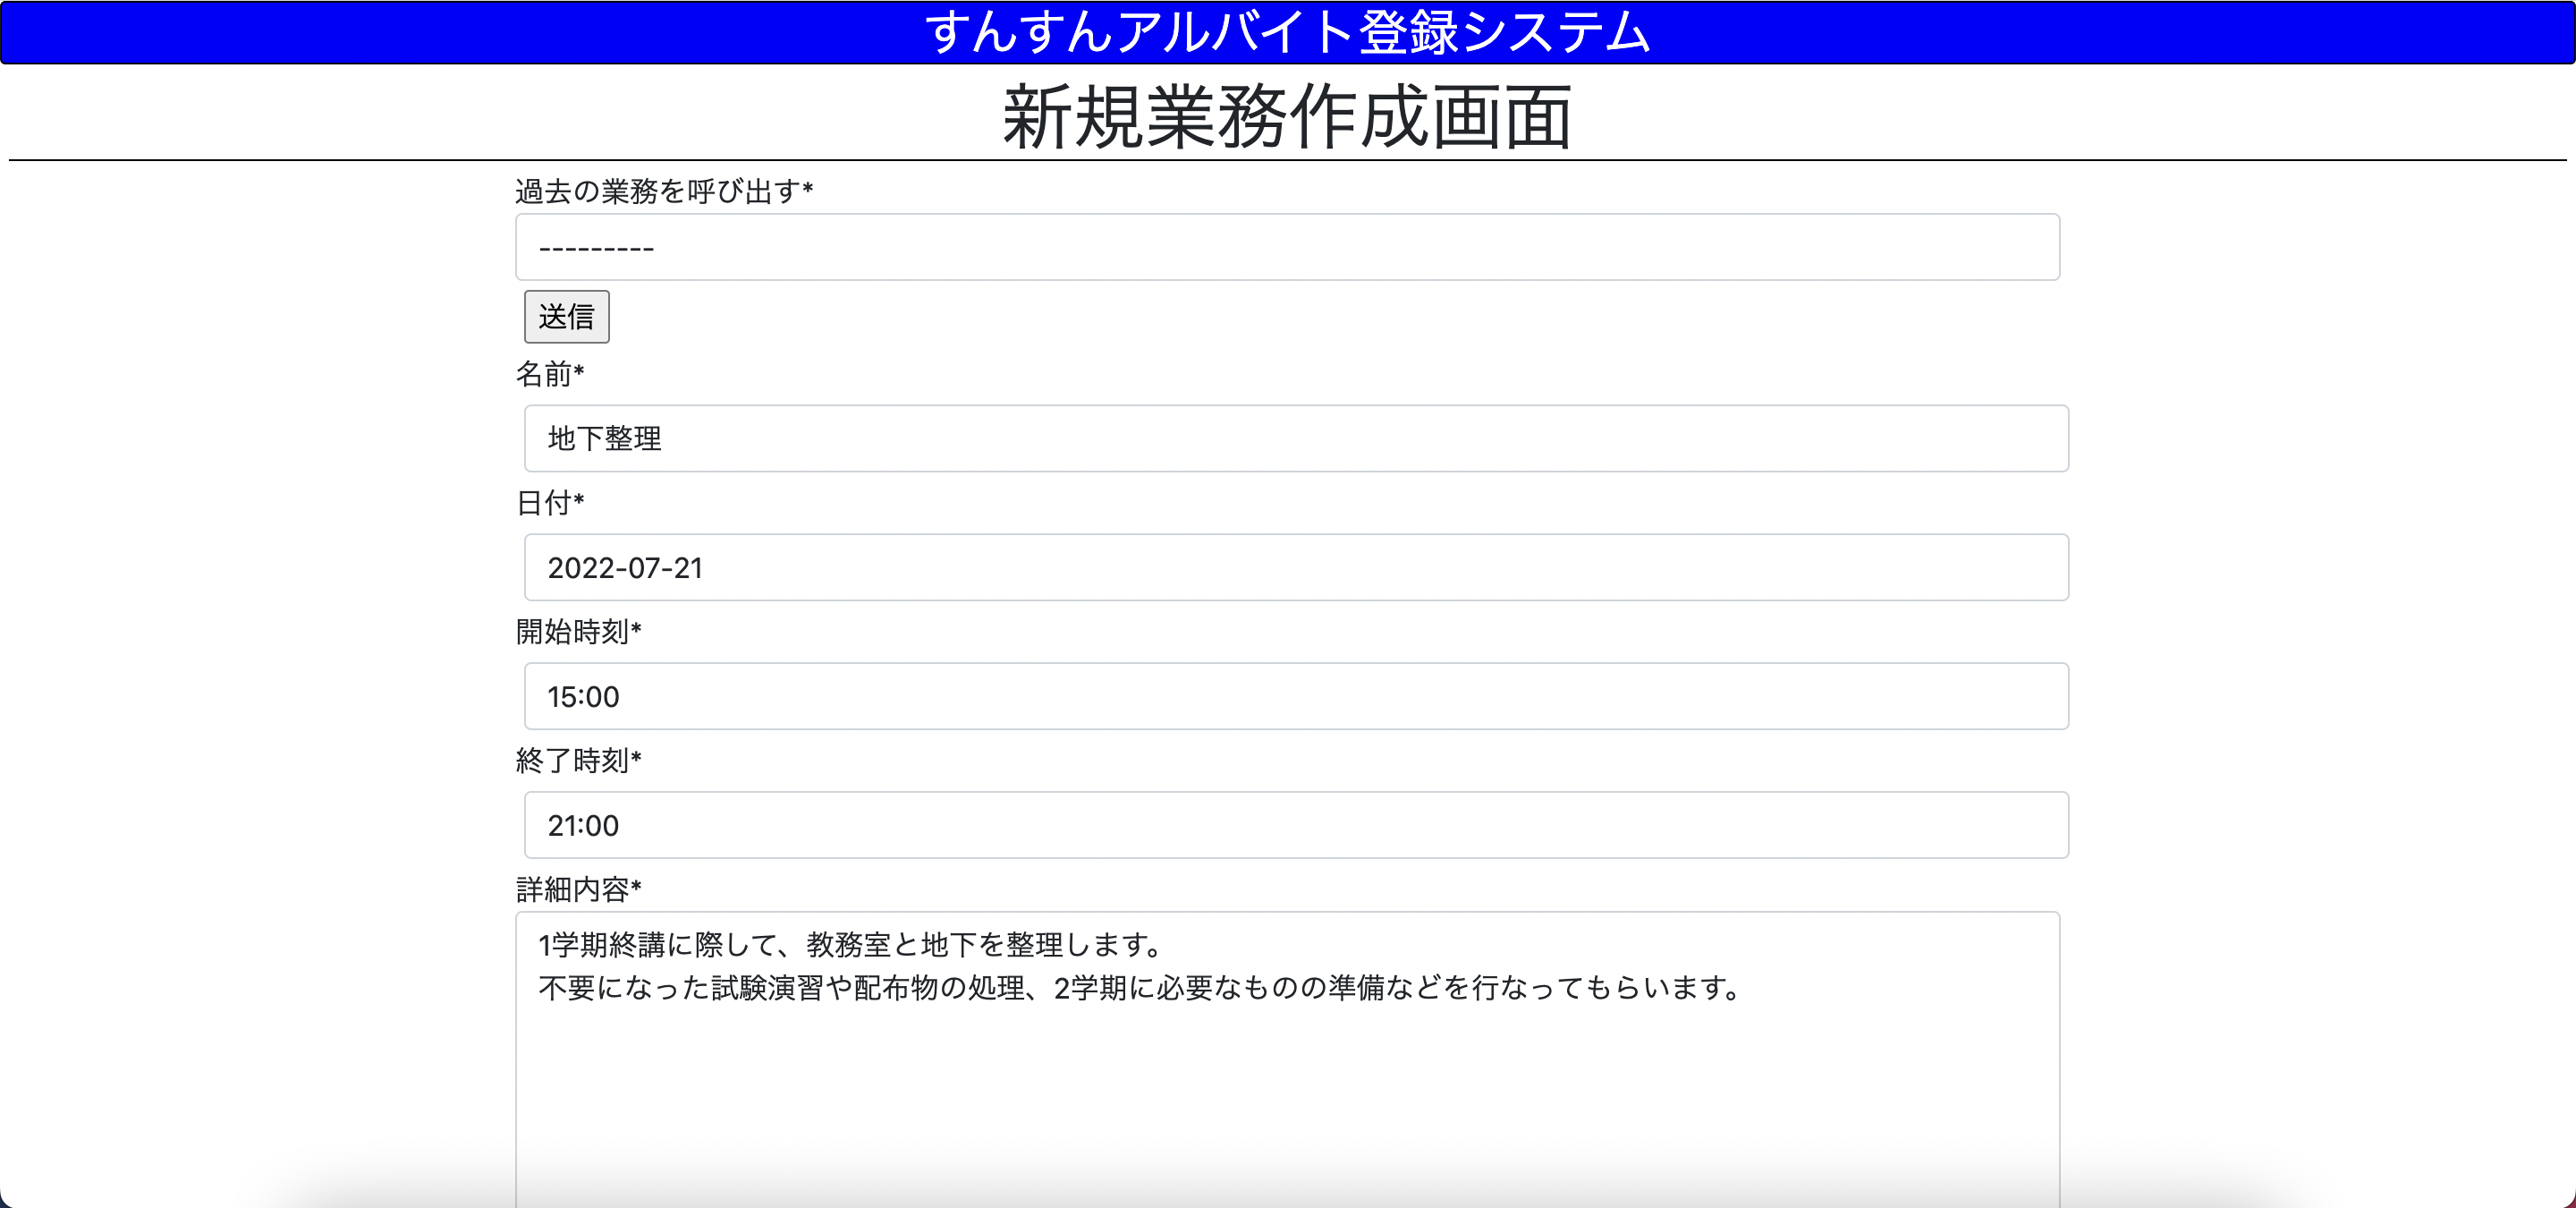
\includegraphics[width=0.8\linewidth]{../figure/6_make_3.png}
				}
			\end{minipage}
		\end{figure}
		一方で業務の作成について、手間を省くために一から全て入力せず過去のものを呼び出すということもできます。
		新規業務作成画面の最上部の「過去の業務を呼び出す」にて、呼び出したい業務を選択・送信することでその業務と同じ情報が自動的に入力されます。
		必要に応じてこれを変更し、業務を作成してください。
		\clearpage


	\subsection{新規従業員登録画面}
		\begin{figure}[htbp]
			\centering
			\fbox{
					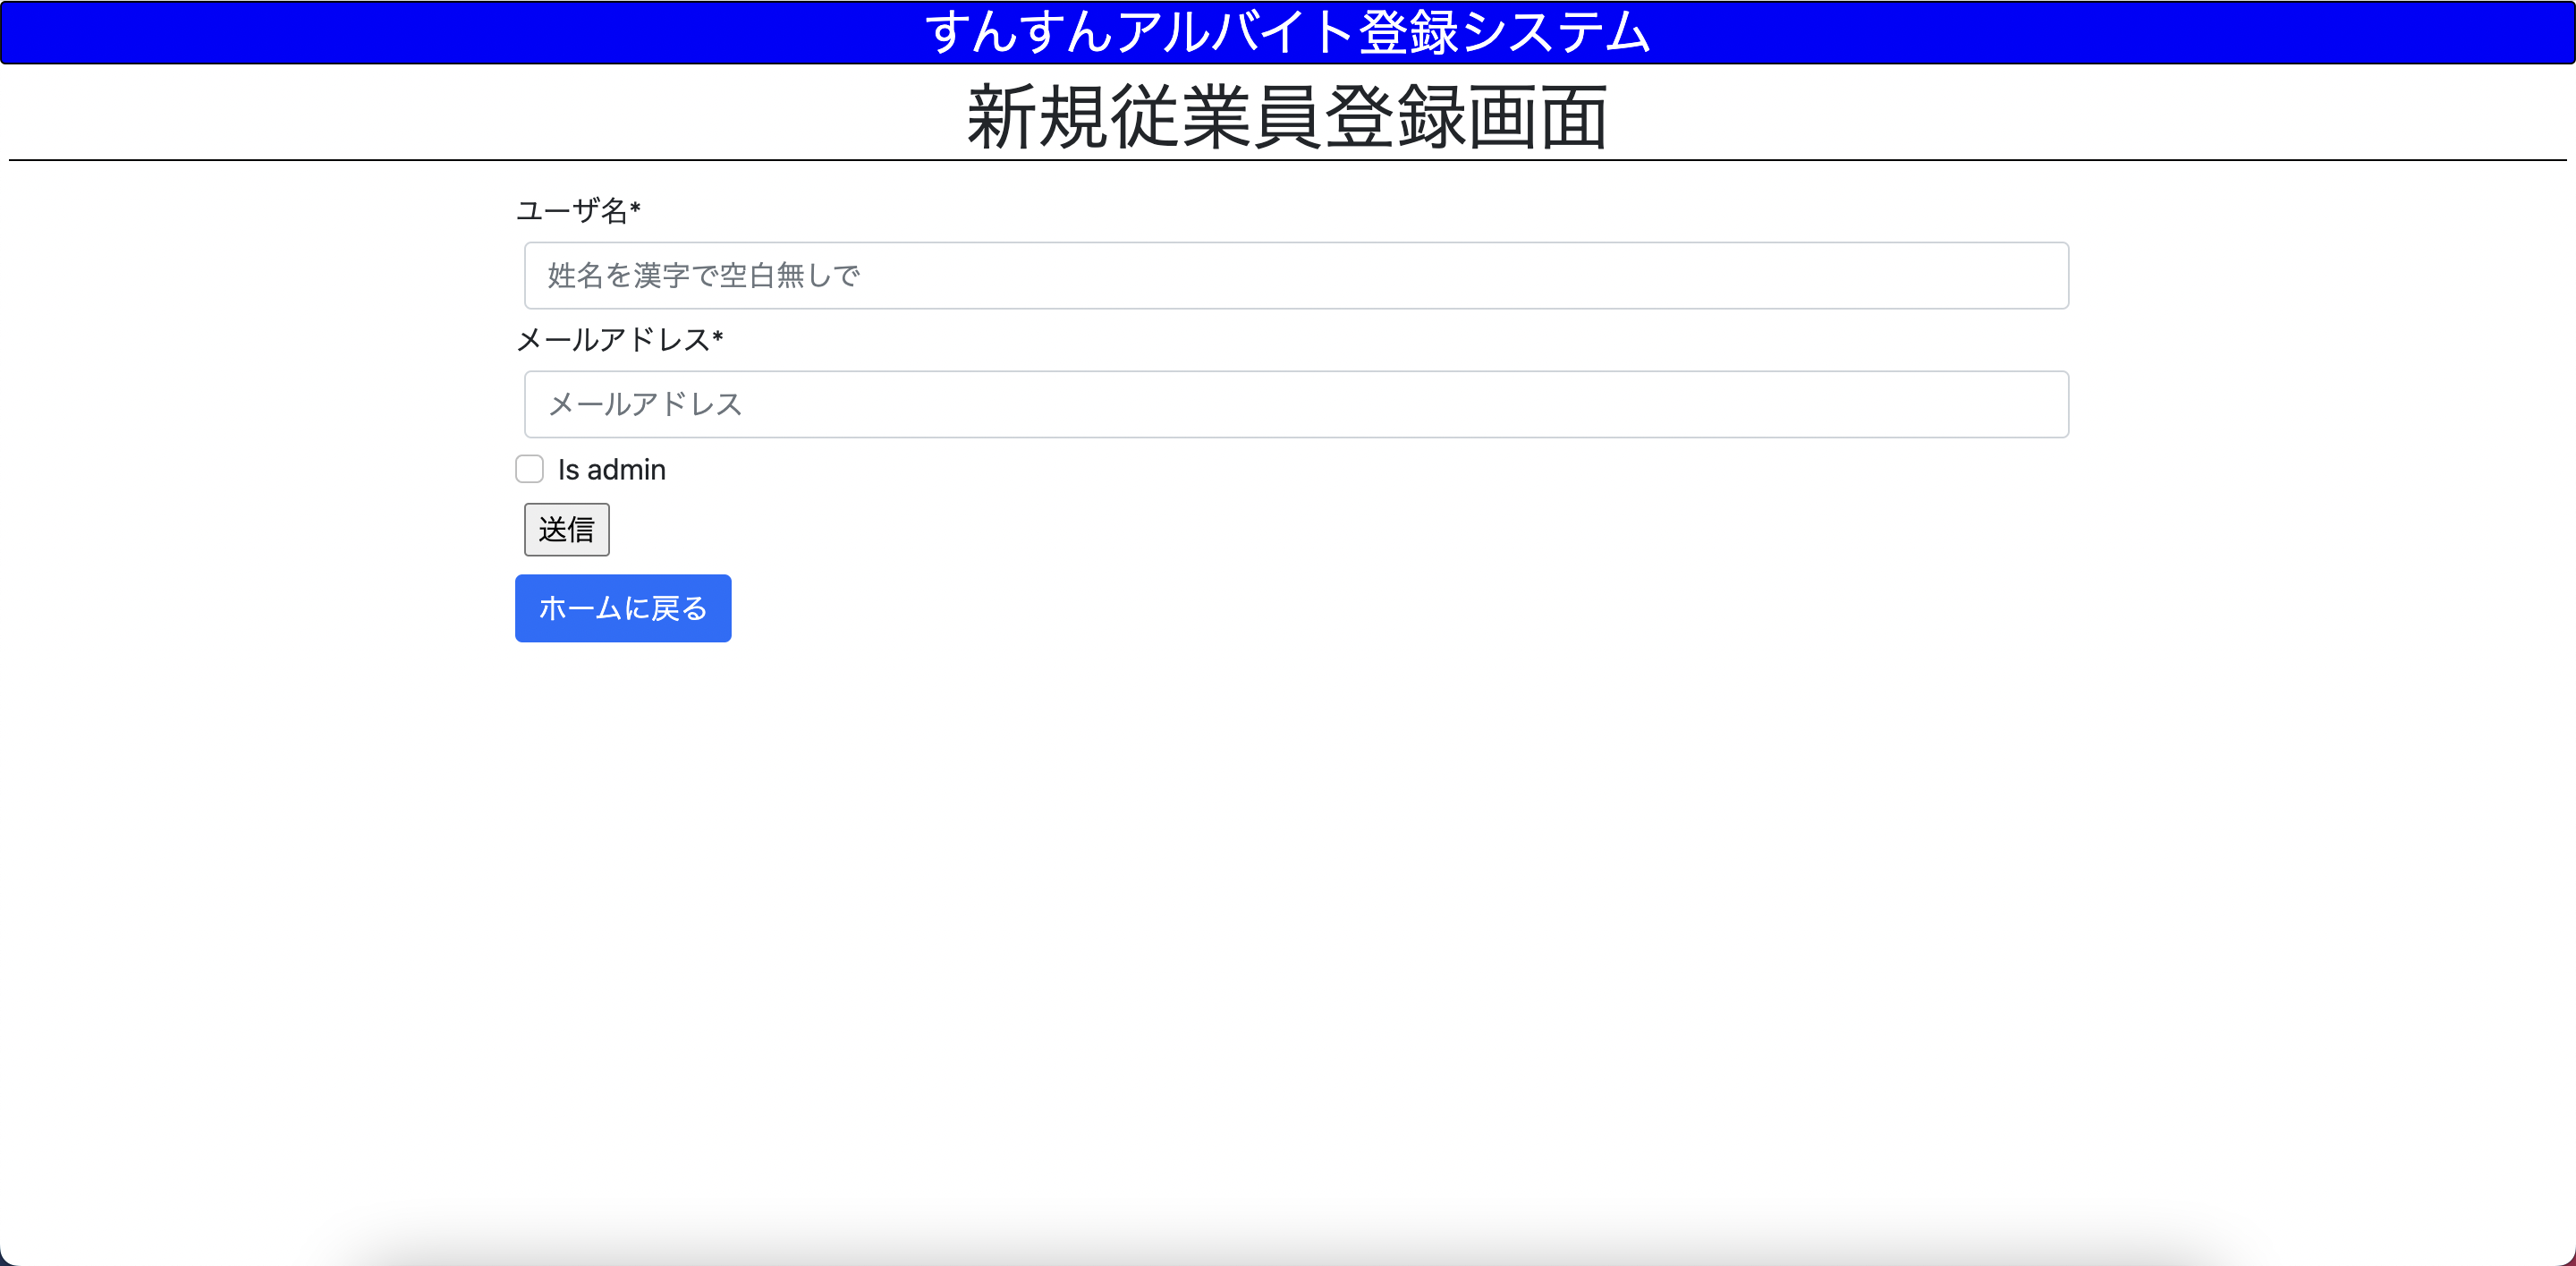
\includegraphics[width=0.8\linewidth]{../figure/7_register.png}
				}
		\end{figure}
		こちらが新規従業員登録画面になります。
		この画面では従業員(社員)の新規登録を行うことができます。
		必要な情報は名前、メールアドレス、社員かどうかの3つです。
		特に名前に関してはログイン画面での認証で用いるので、正確に記入して下さい。
		社員を登録する場合は「is admin」にチェックを入れてください。
		\par

		従業員は登録されると初期パスワードとして「0000」が配布されます。
		新たに登録した際はこの旨を各従業員にお伝え下さい。


	\subsection{従業員削除画面}
		\begin{figure}[htbp]
			\centering
			\fbox{
					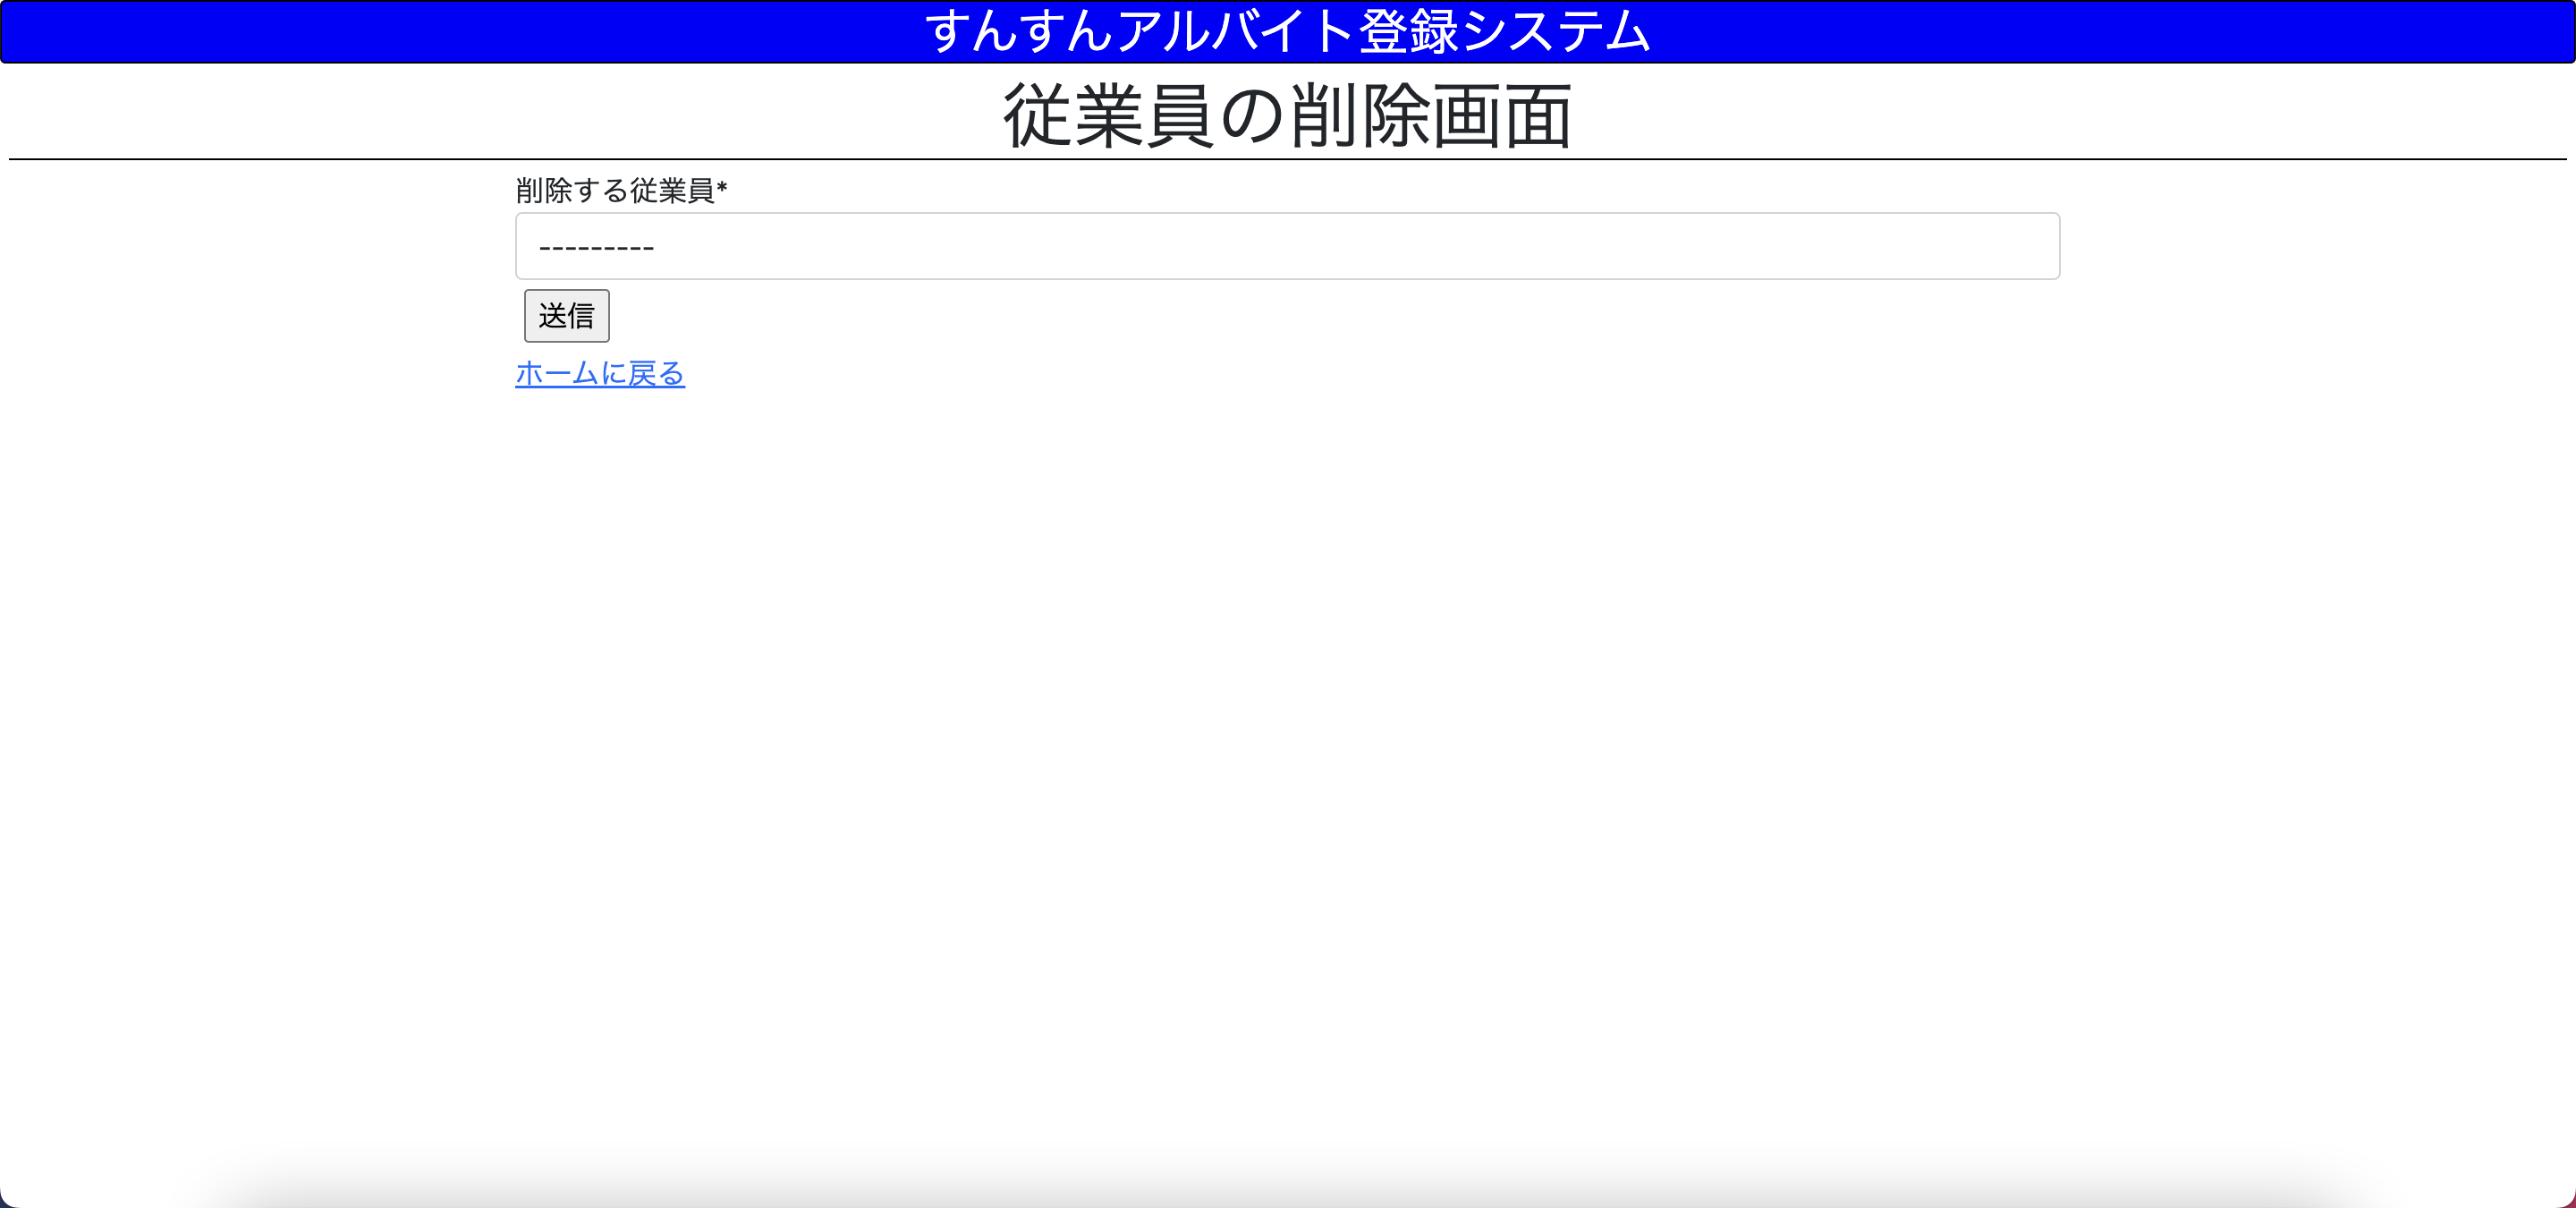
\includegraphics[width=0.8\linewidth]{../figure/8_delete.png}
				}
		\end{figure}
		こちらが従業員削除画面になります。
		卒業や異動で従業員を削除したい場合に利用して下さい。
		また今後勤務予定の業務がある従業員を削除することはできないようにしております。
	\clearpage


\section{従業員の操作方法}
	\subsection{ホーム画面}
		\begin{figure}[htbp]
			\centering
			\fbox{
					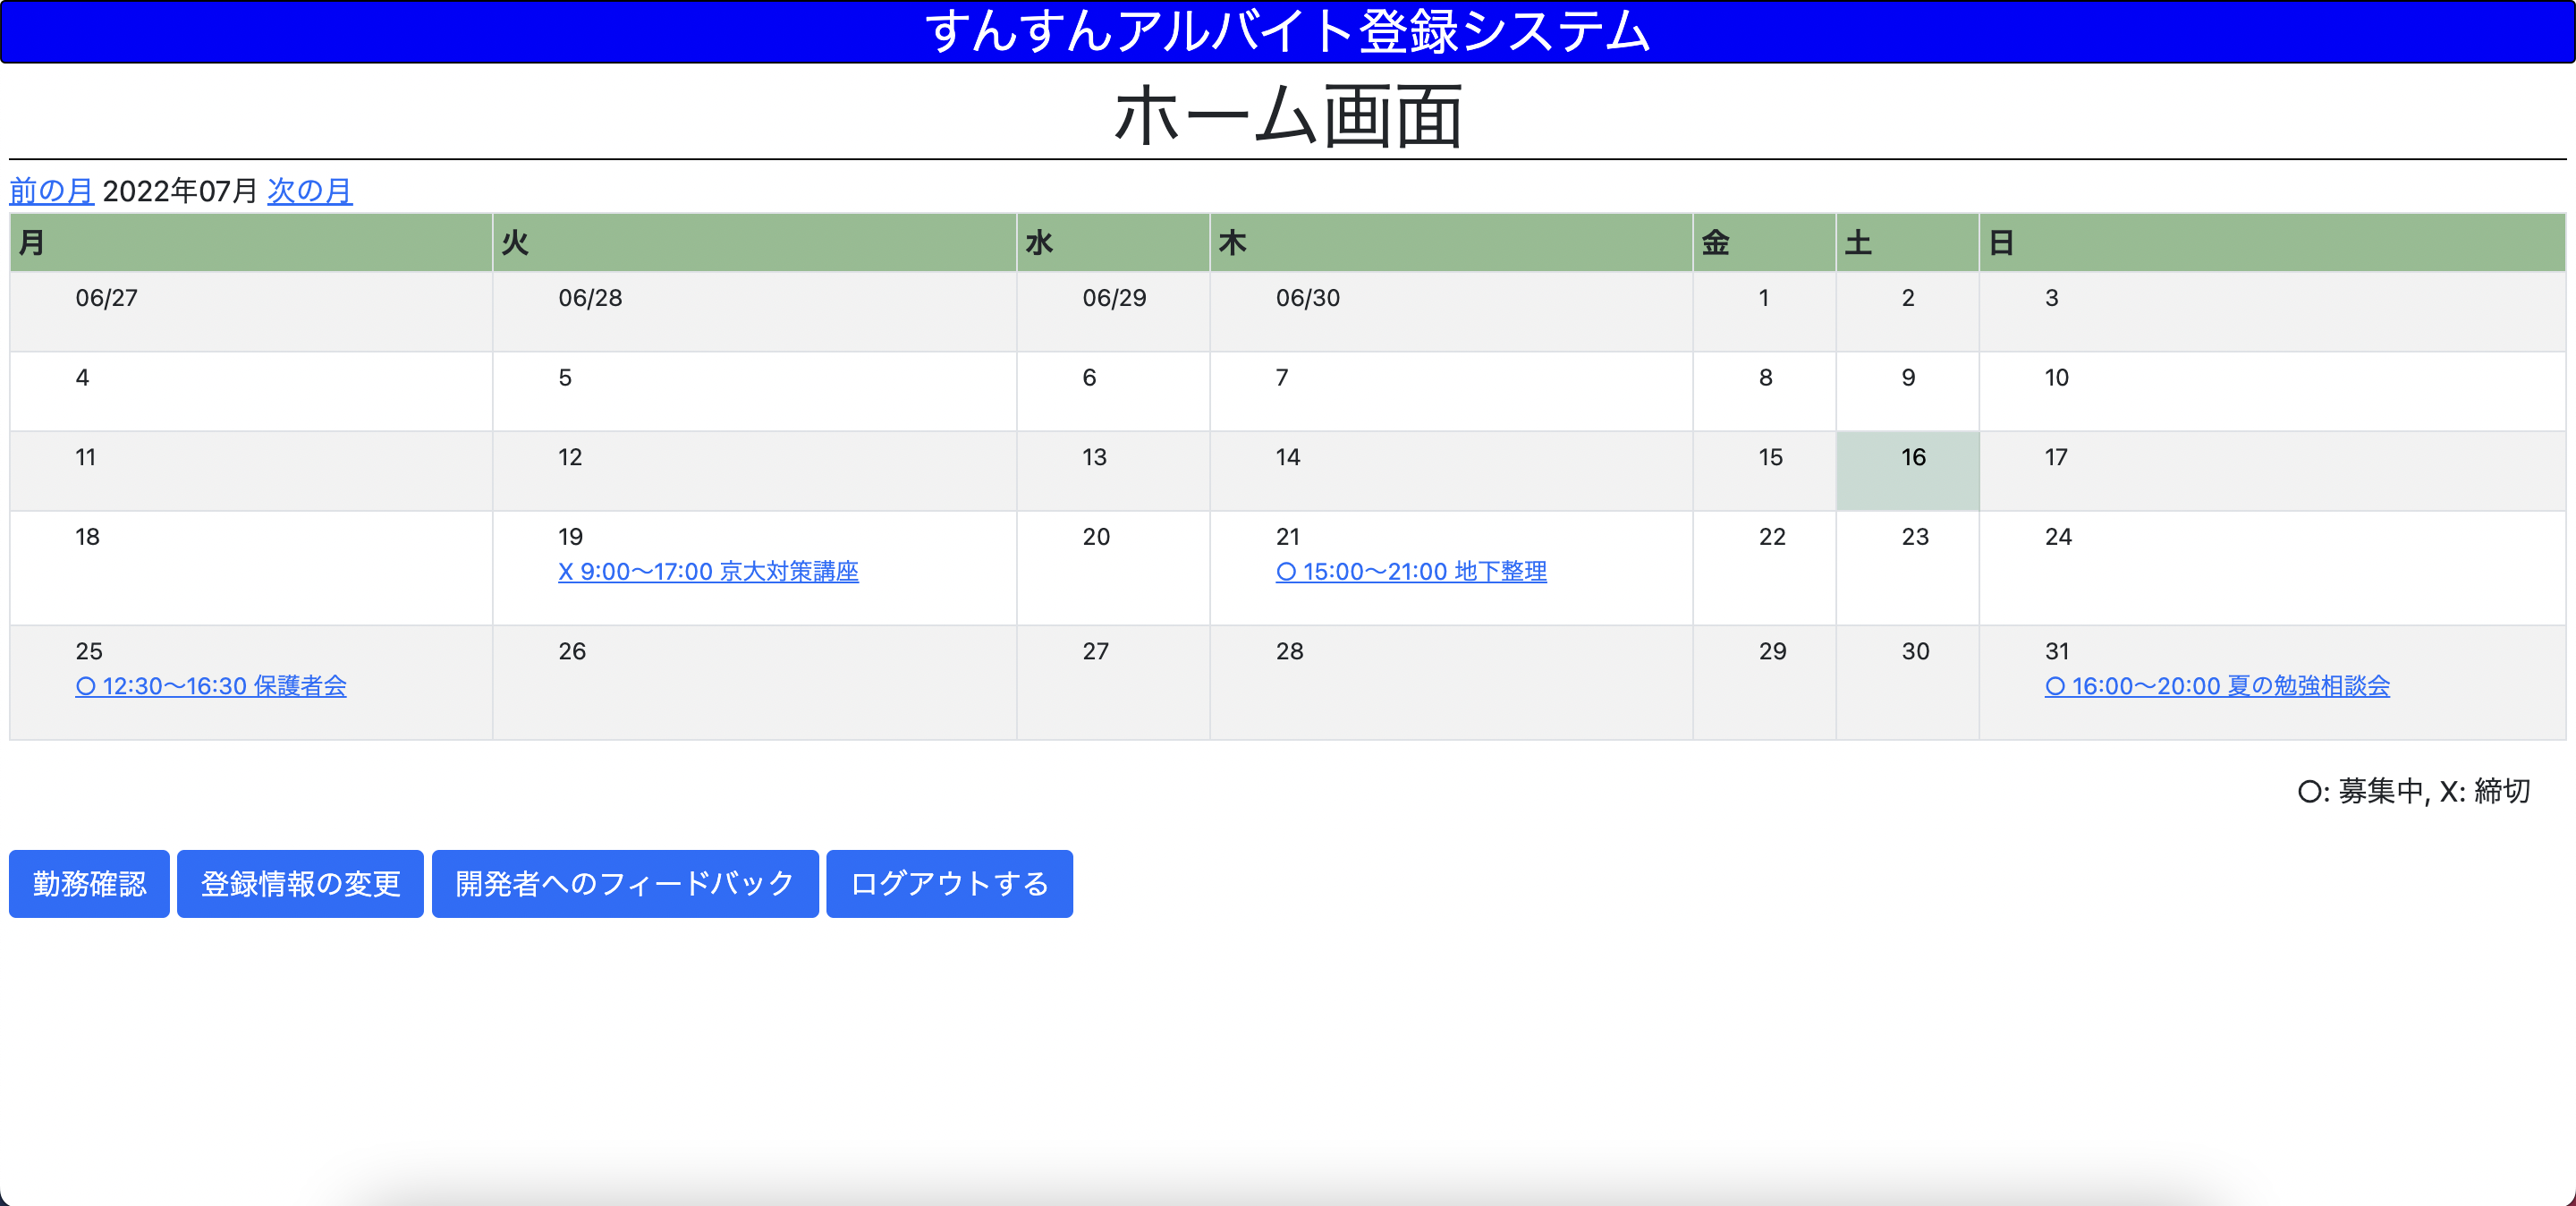
\includegraphics[width=0.8\linewidth]{../figure/11_home_non.png}
				}
		\end{figure}
		こちらが従業員用のホーム画面になります。
		カレンダーについては社員用と同様に業務をクリックすることでその詳細画面に遷移することができます(3.3を参照)。
		一方で業務の作成などの権限は無く、代わりに勤務確認というボタンがあります(3.2を参照)。

	\subsection{勤務確認画面}
		\begin{figure}[htbp]
			\centering
			\fbox{
					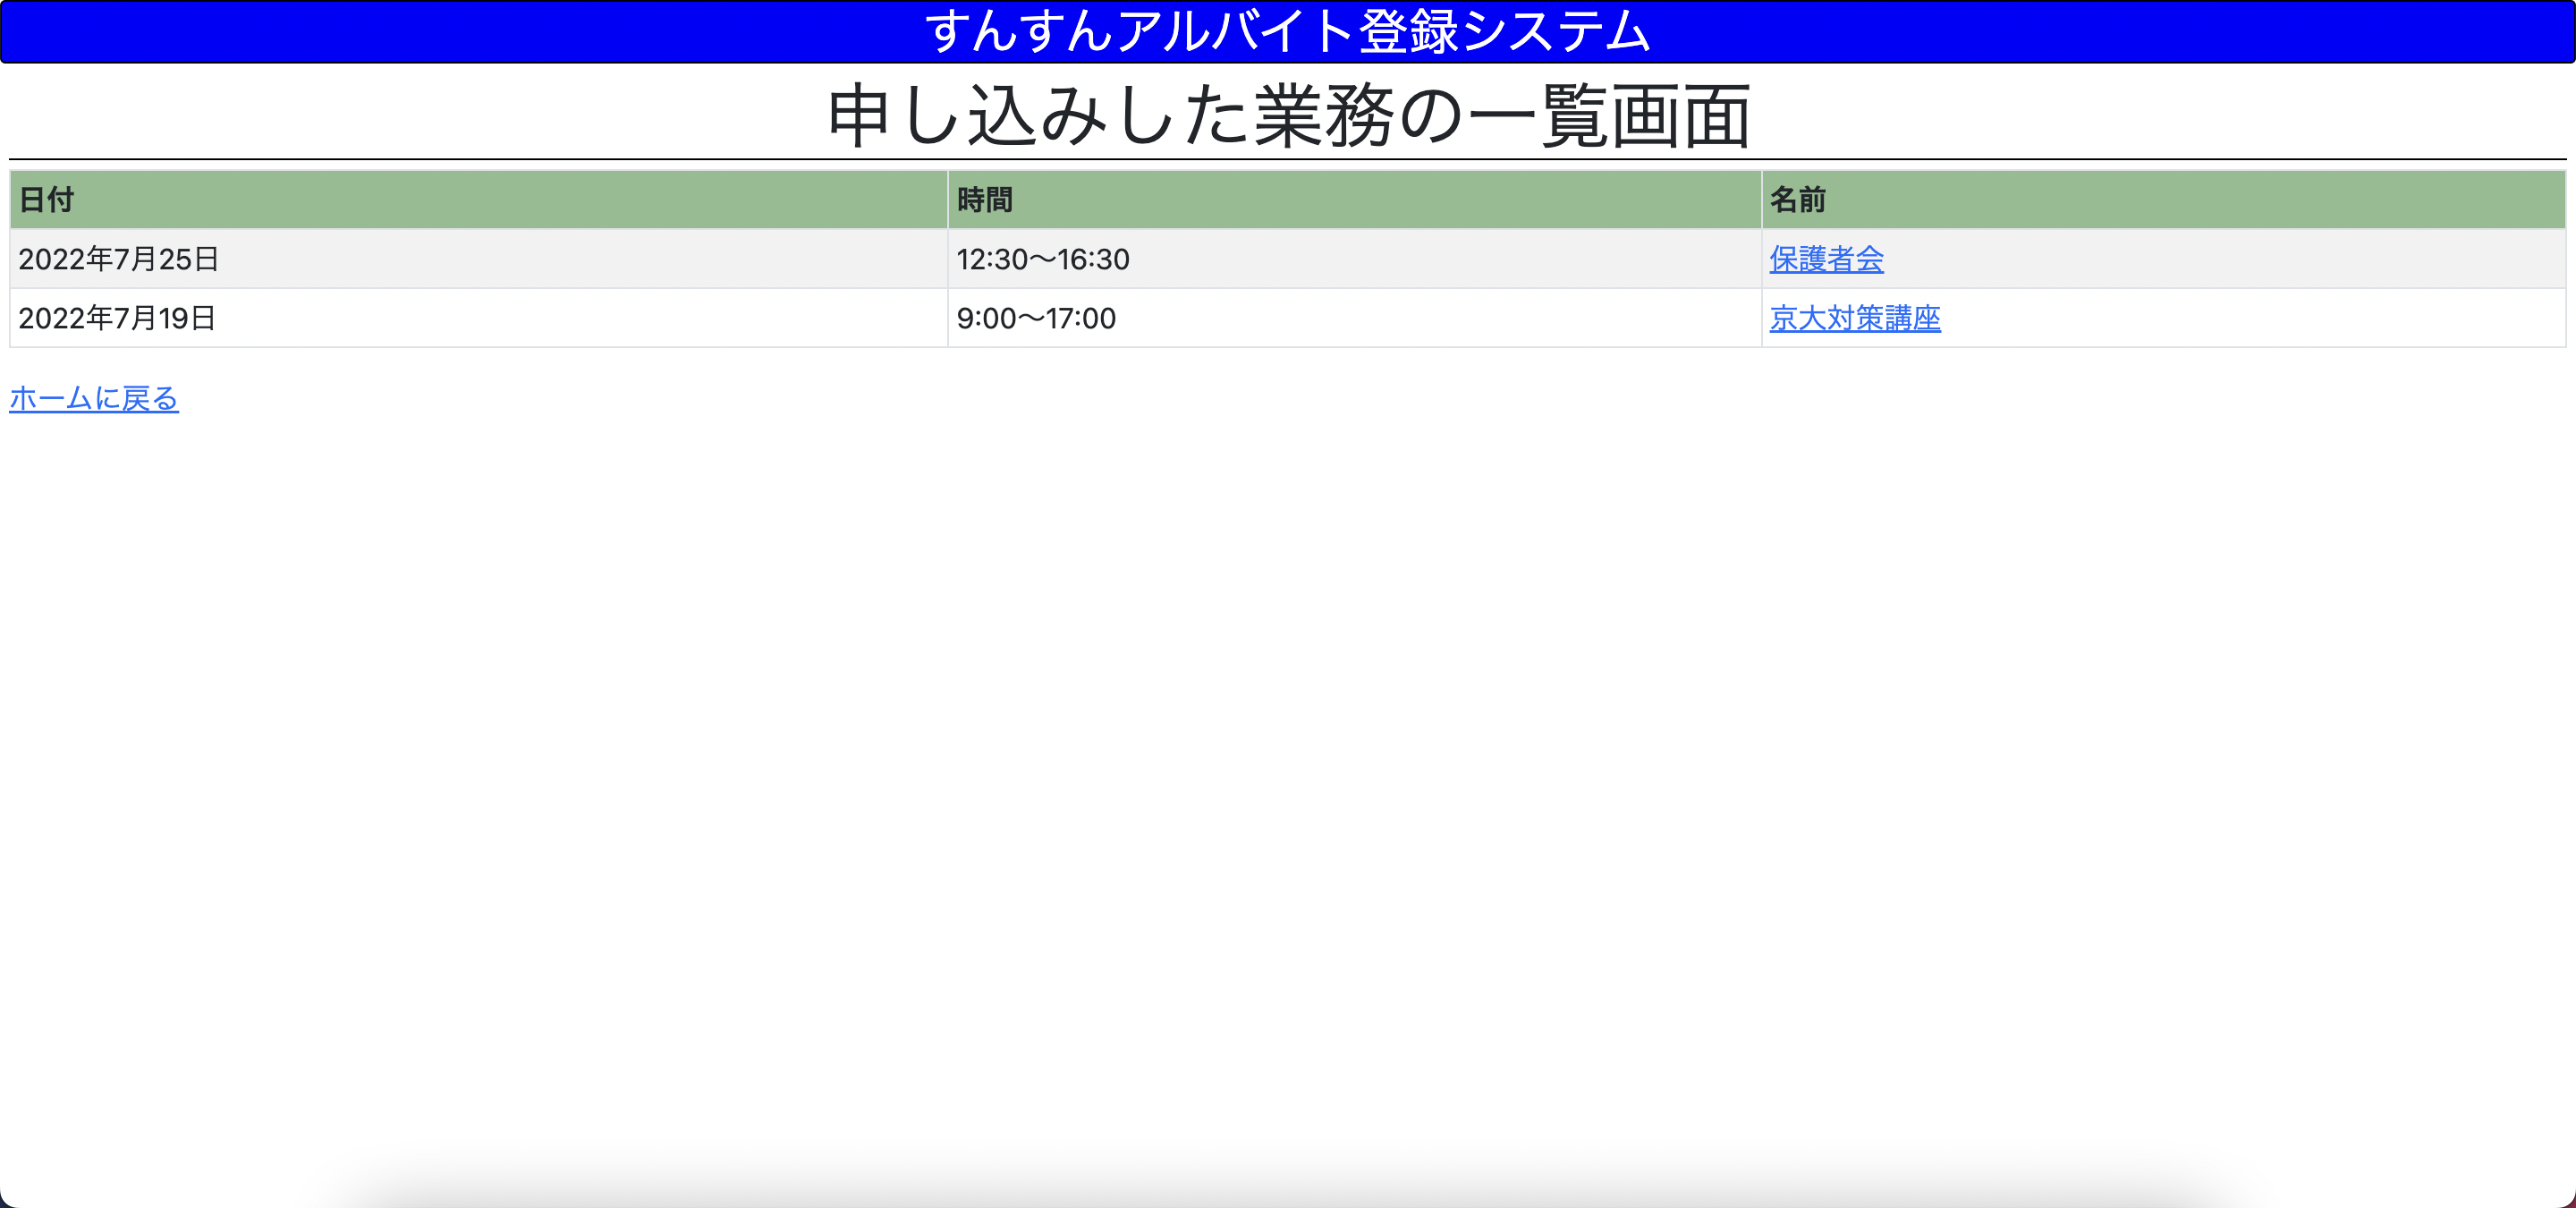
\includegraphics[width=0.8\linewidth]{../figure/12_confirm.png}
				}
		\end{figure}
		こちらが勤務確認画面になります。
		従業員は自分が過去に申し込んだ業務を知ることができます。
		右端にある業務名をクリックすることで、ホーム画面と同様にその業務の詳細画面へと遷移できます。
		\clearpage

	\subsection{業務詳細画面}
		\begin{figure}[htbp]
			\begin{minipage}[b]{\linewidth}
				\centering
				\fbox{
					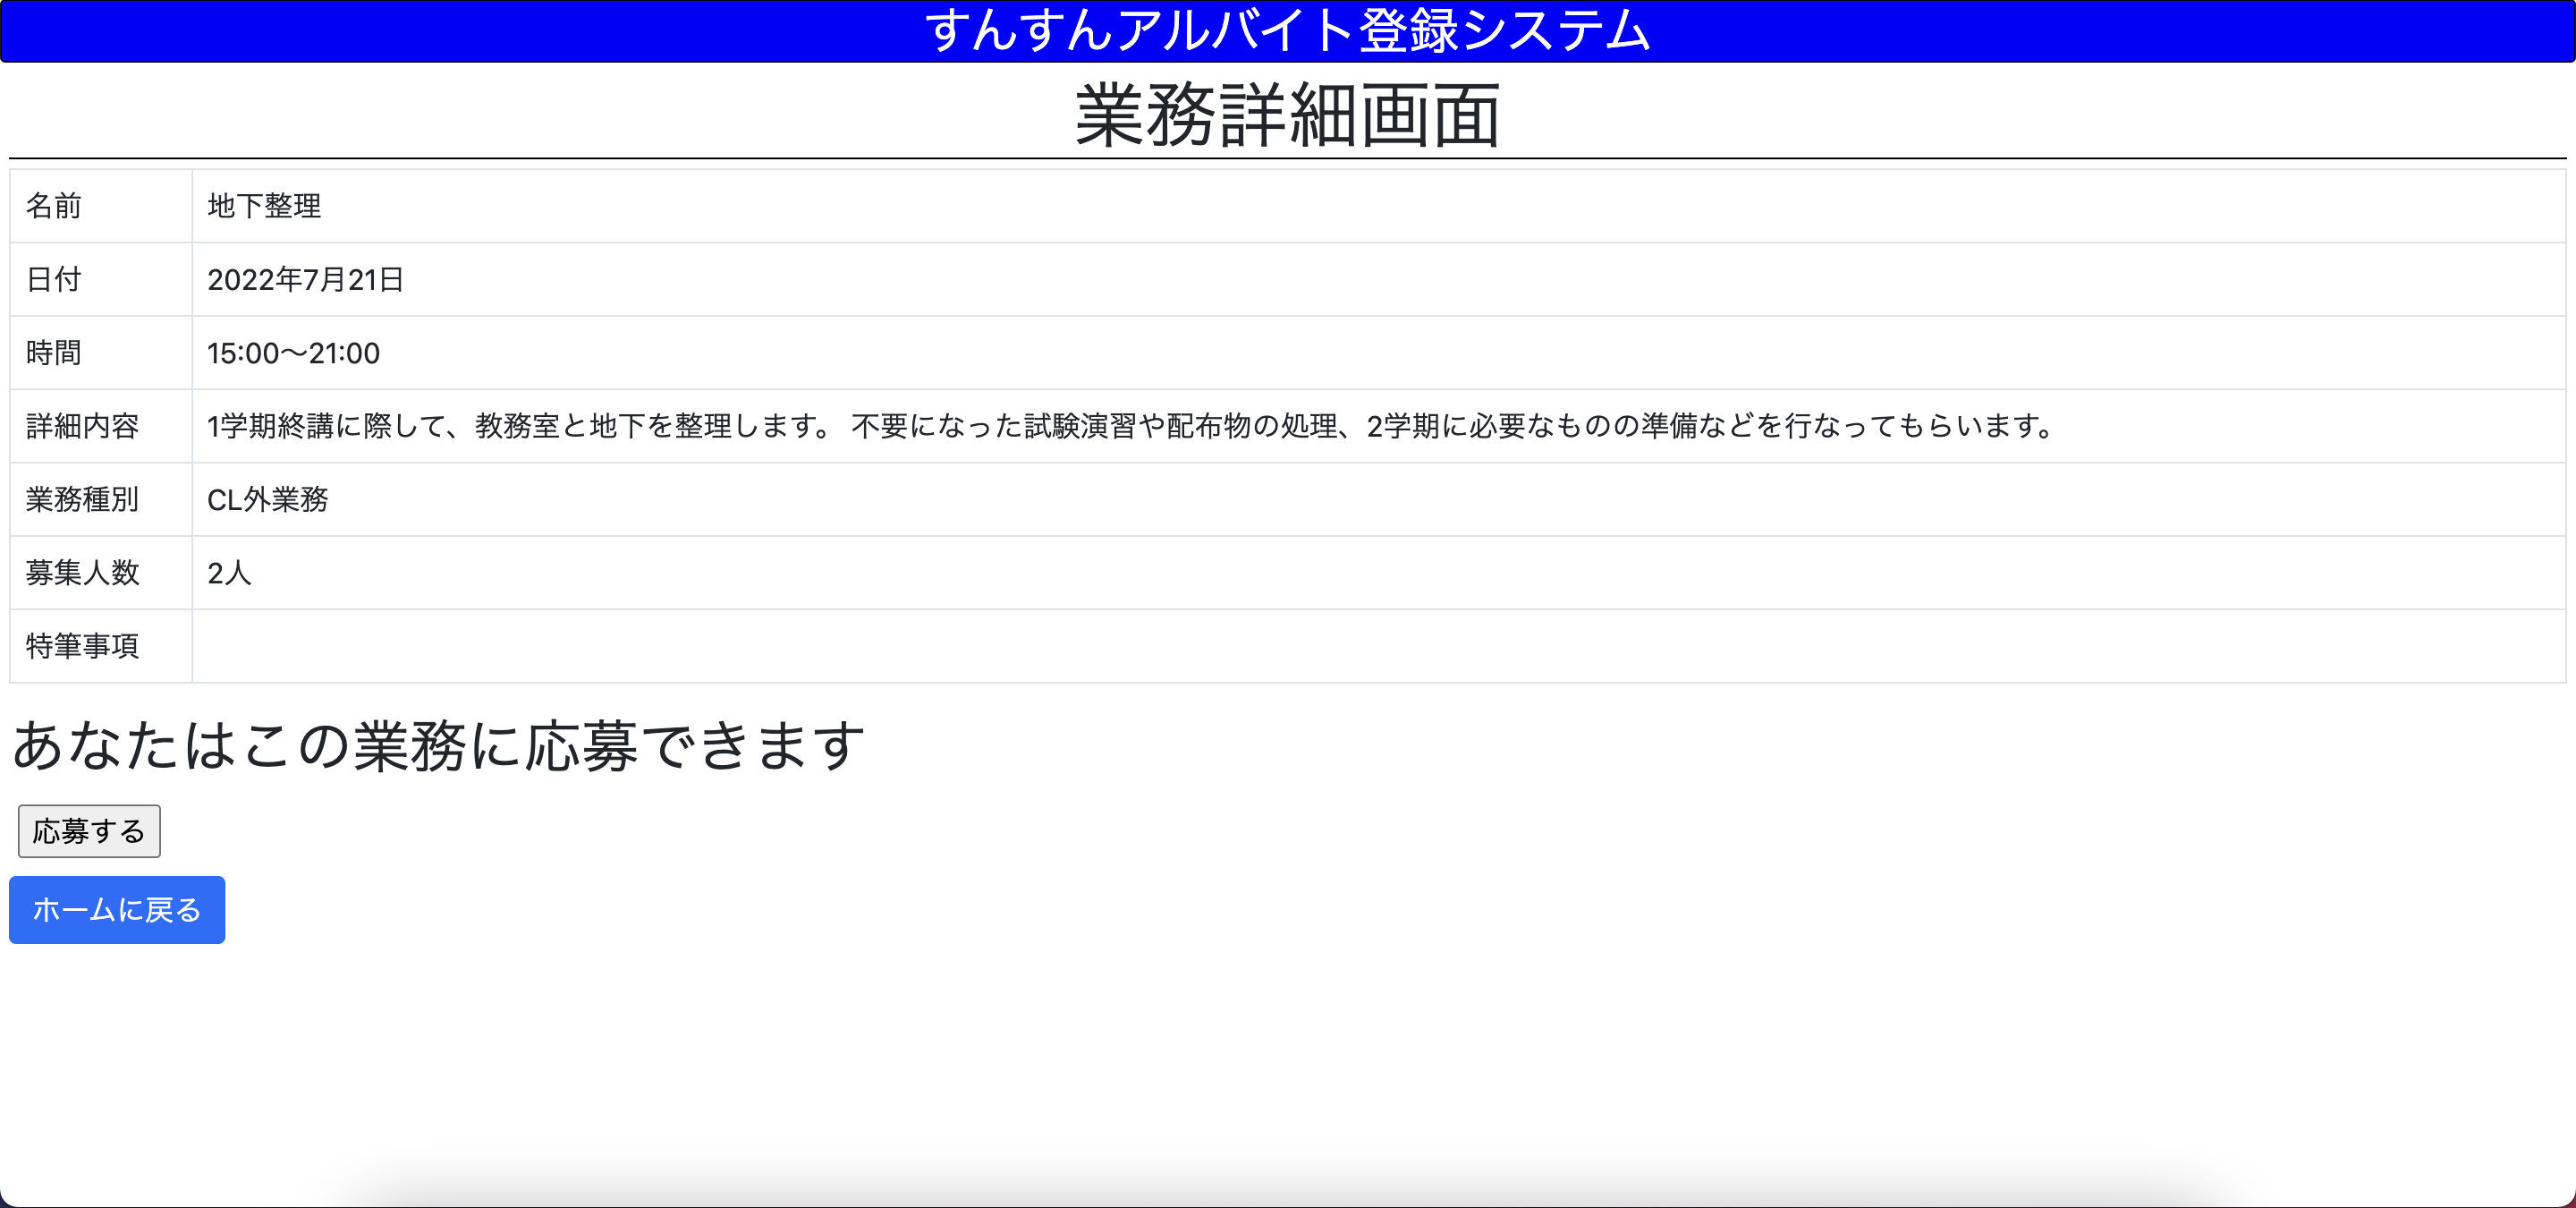
\includegraphics[width=0.8\linewidth]{../figure/13_specification_non_1.png}
				}
			\end{minipage} \\
			\begin{minipage}[b]{\linewidth}
				\centering
				\fbox{
					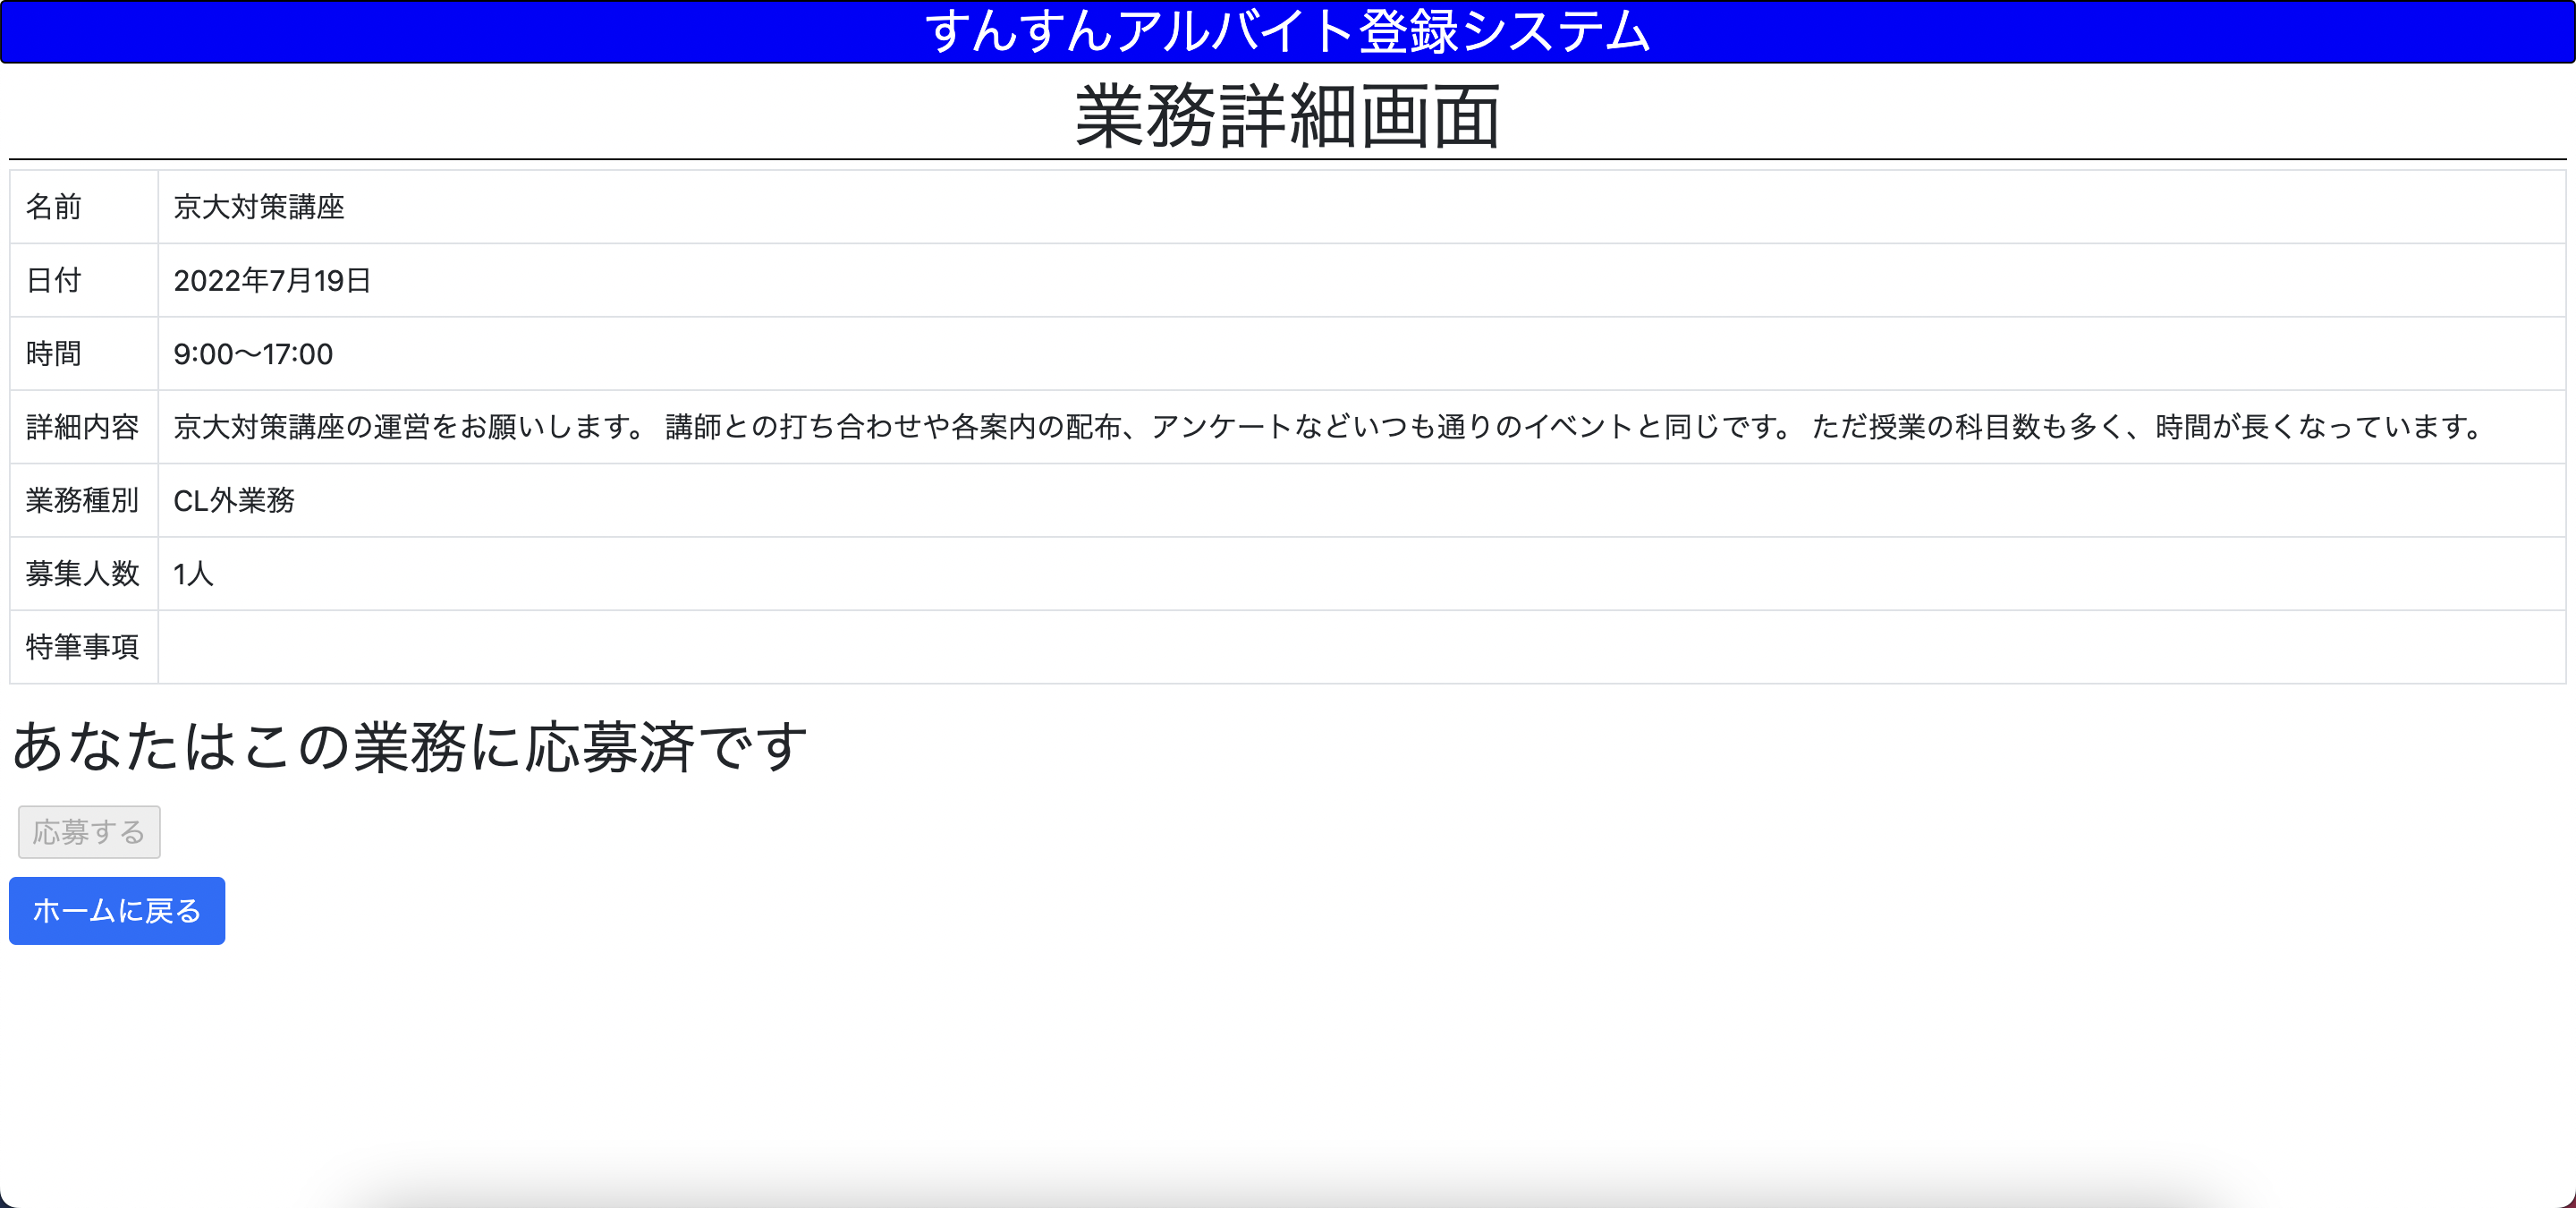
\includegraphics[width=0.8\linewidth]{../figure/13_specification_non_2.png}
				}
			\end{minipage}
		\end{figure}
		こちらが従業員用の業務詳細画面になります。
		詳細内容が表形式で提示されるとともに、従業員はこの画面から業務へ応募することができます。
		業務が定員に達した、もしくは既に応募したものについては送信ボタンが押せないように設計しております。
		社員用の画面と違って、従業員は他に誰が応募しているか知ることはできないようになっております。
		\clearpage


\section{従業員に送信されるメール}
	\subsection{応募完了通知}
		\begin{figure}[htbp]
			\centering
			\fbox{
					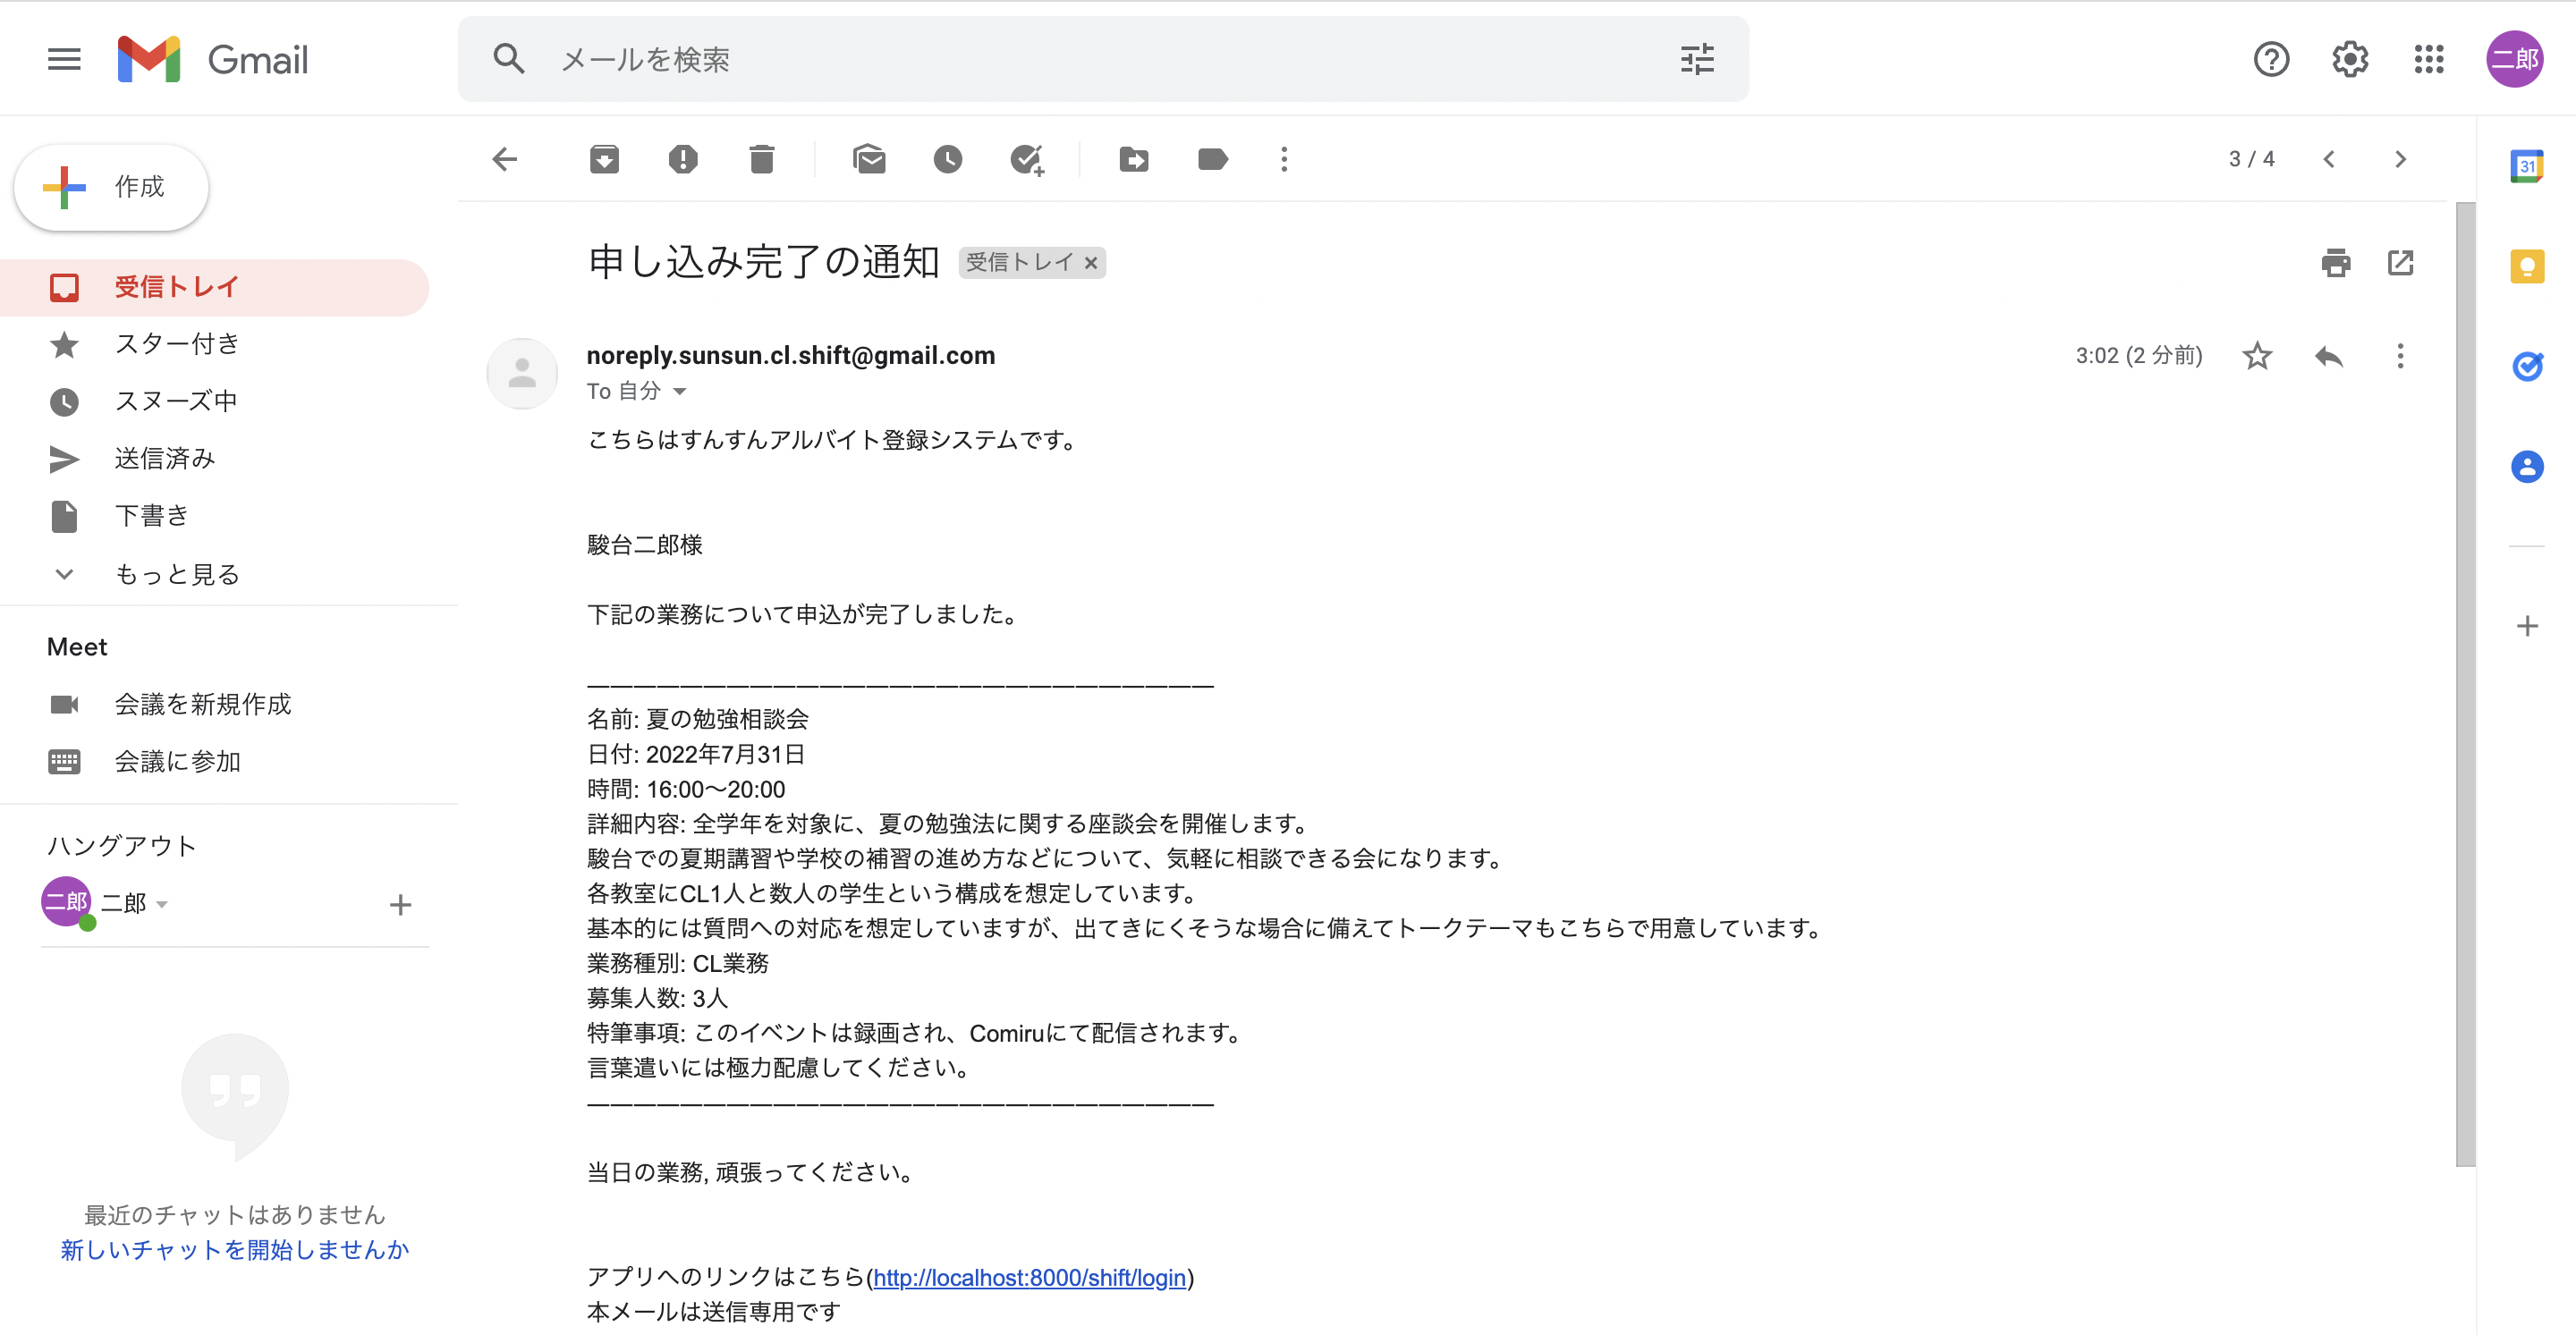
\includegraphics[width=0.8\linewidth]{../figure/14_mail_1.png}
				}
		\end{figure}
		従業員が業務詳細画面から応募した際、このメールが自動で送信されます。

	\subsection{募集開始通知}
		\begin{figure}[htbp]
			\centering
			\fbox{
					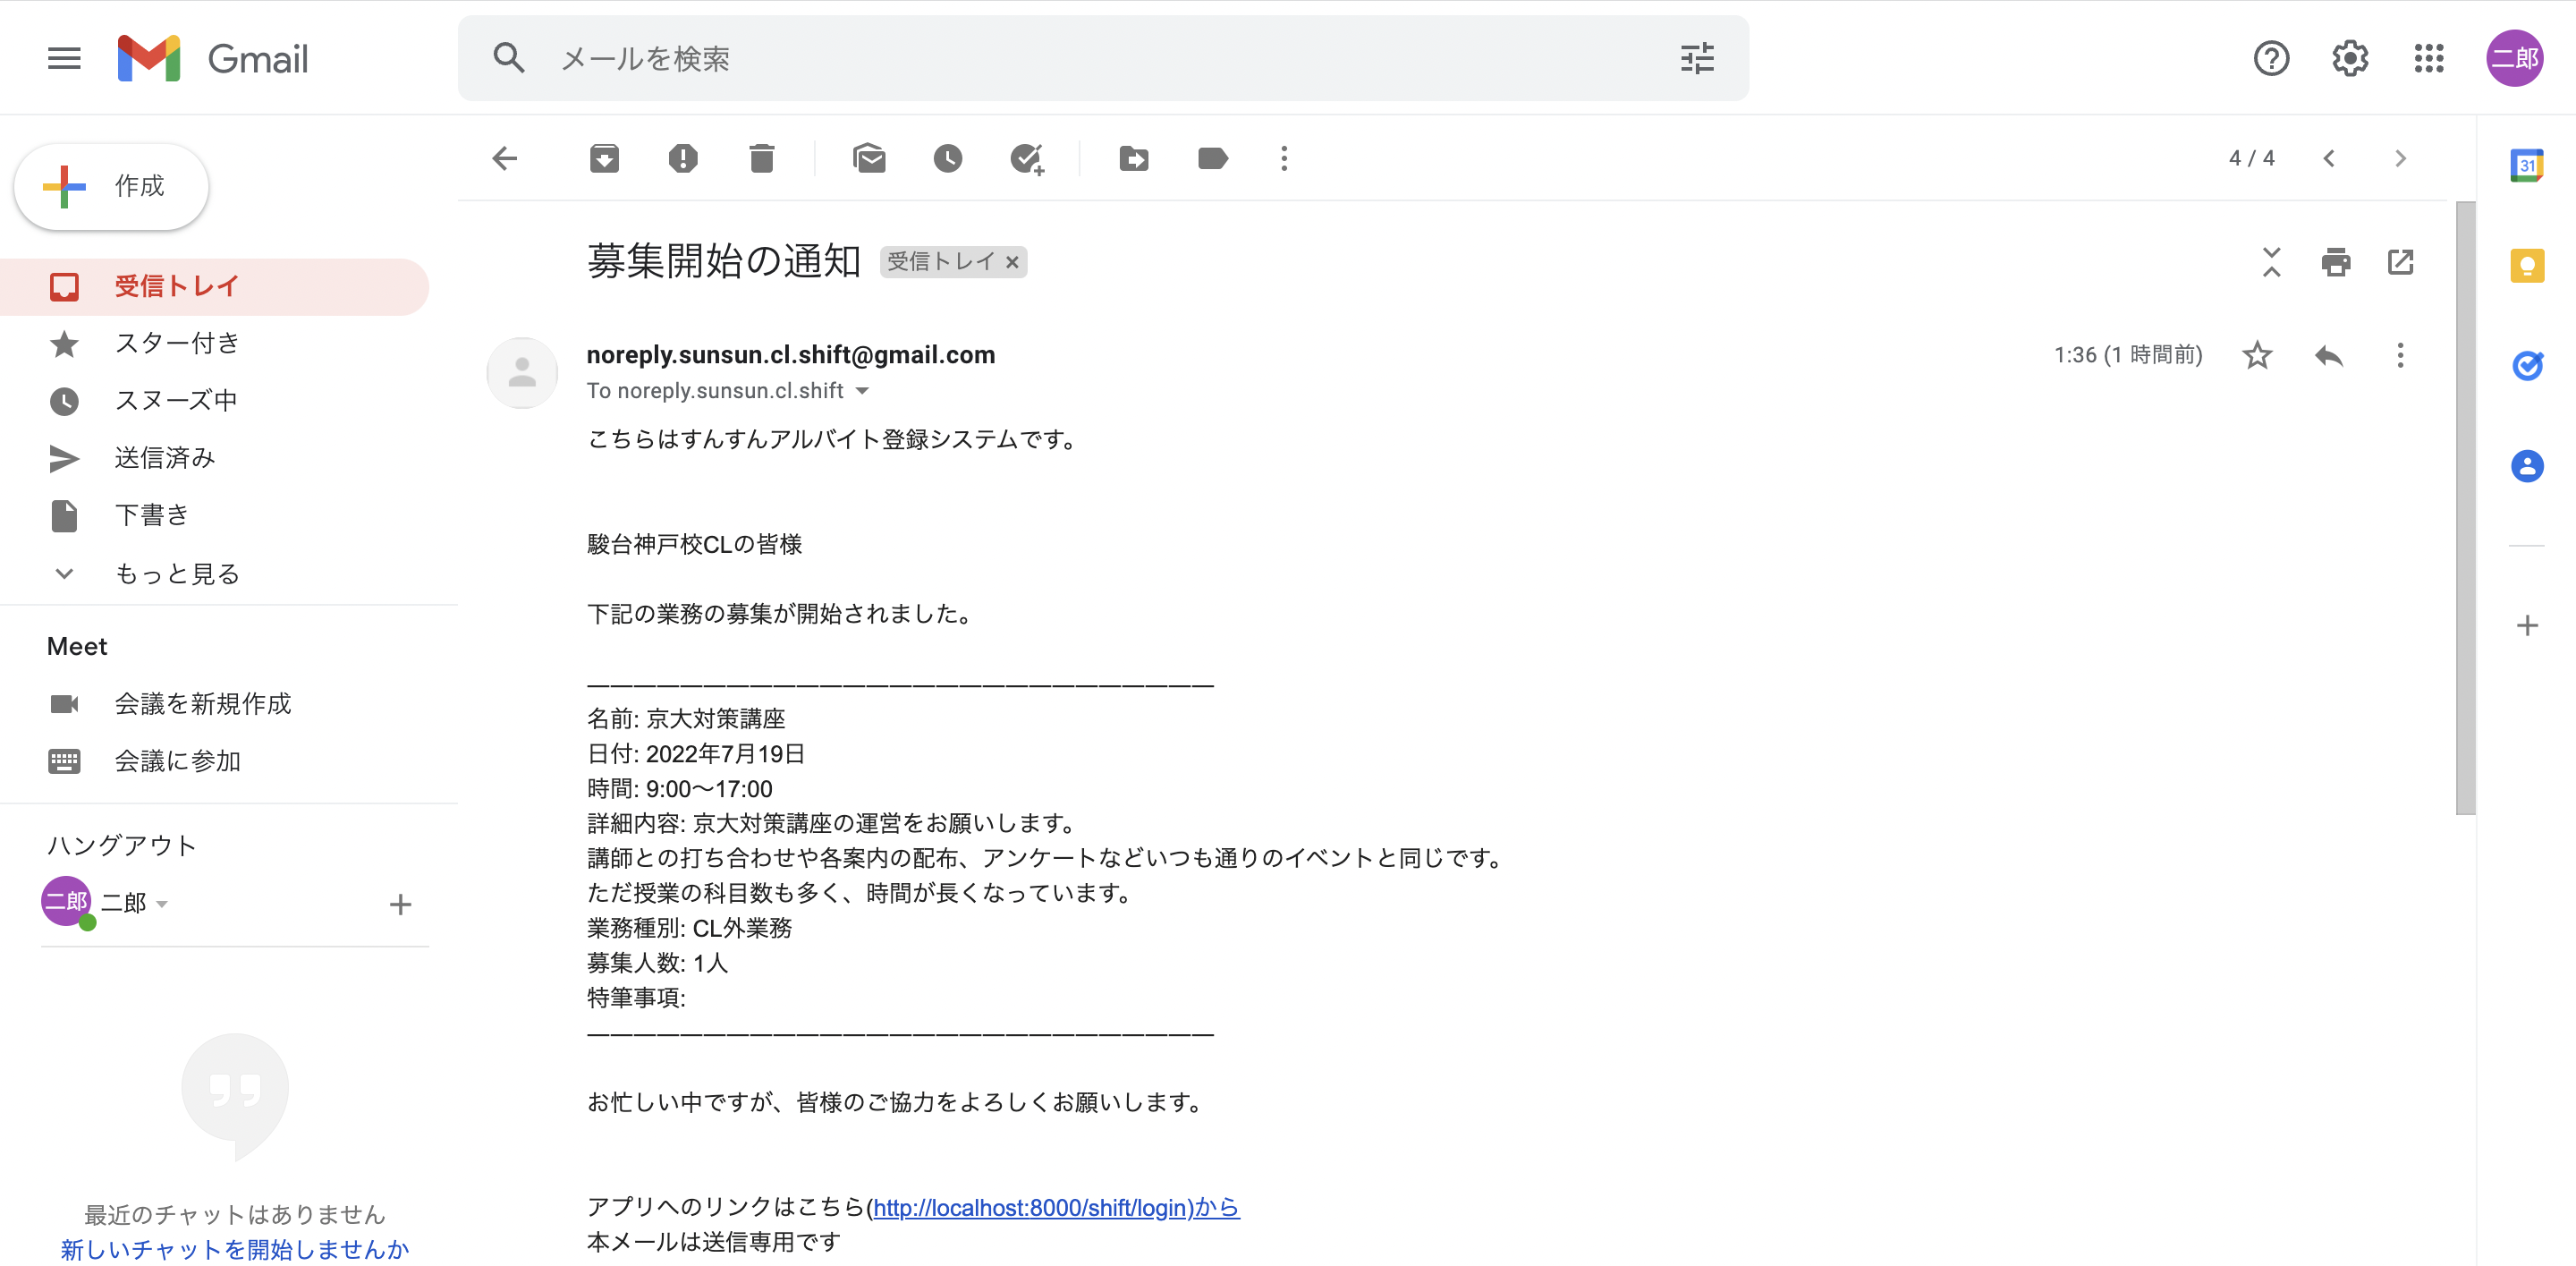
\includegraphics[width=0.8\linewidth]{../figure/14_mail_2.png}
				}
		\end{figure}
		社員が新規業務作成画面にて業務を作成した際に、このメールが全従業員宛にBCCで送信されます。

	\subsection{出勤前日のリマインド}
		\begin{figure}[htbp]
			\centering
			\fbox{
					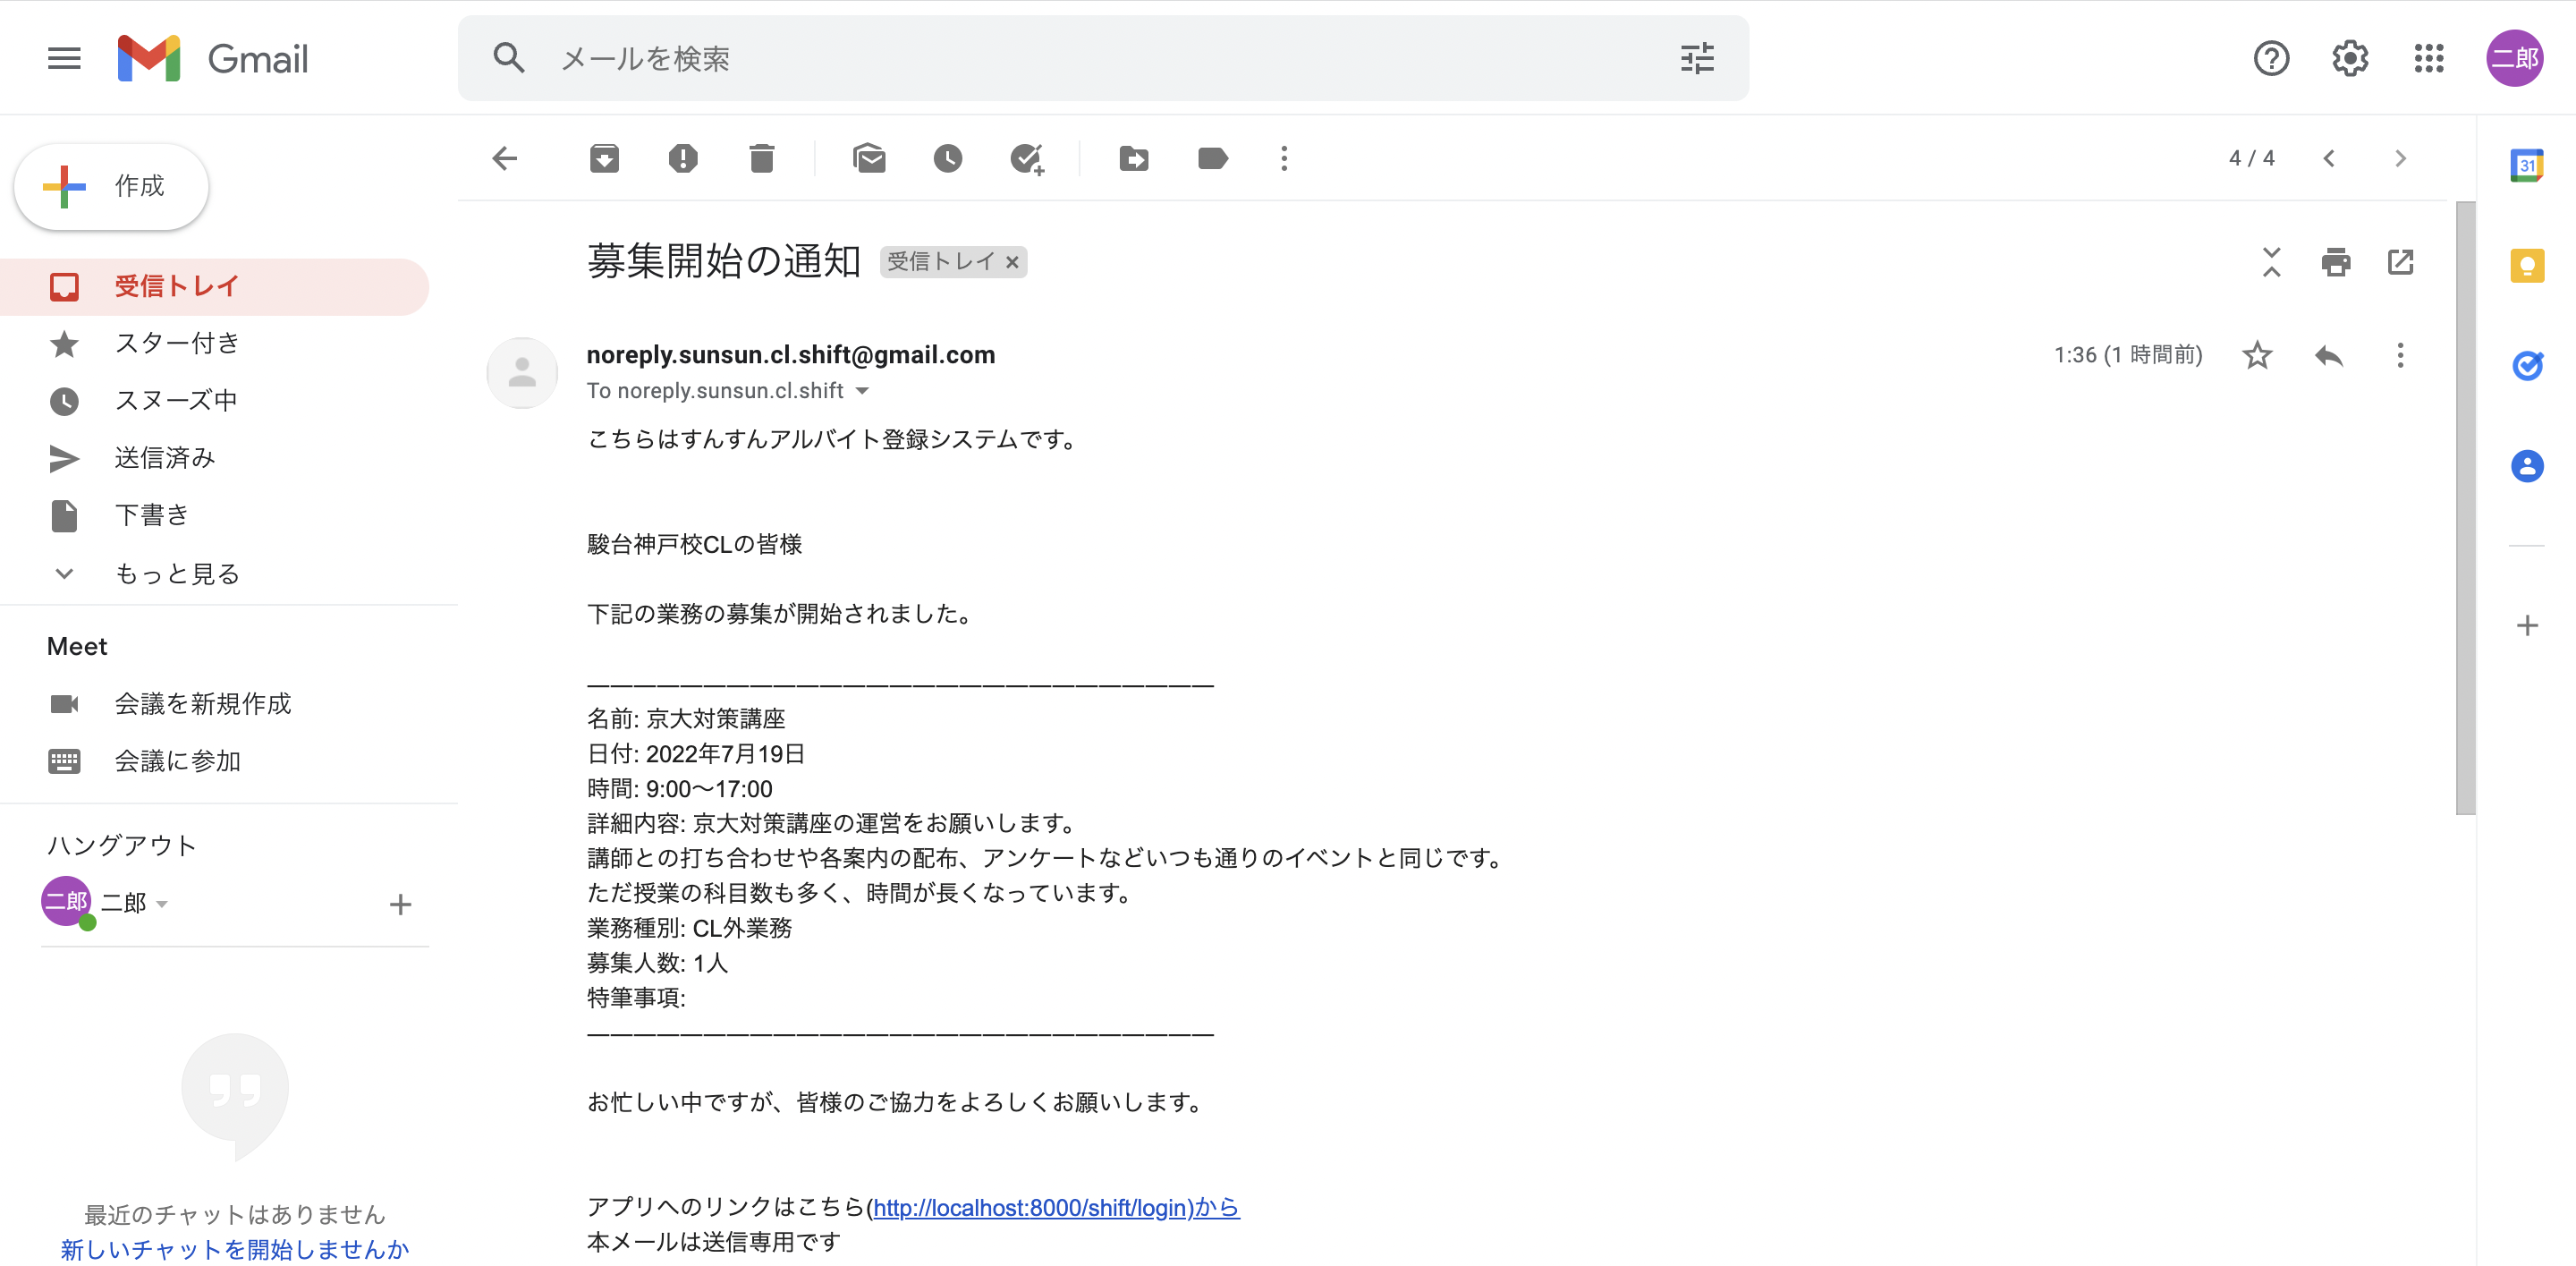
\includegraphics[width=0.8\linewidth]{../figure/14_mail_2.png}
				}
		\end{figure}
		次の日に出勤がある従業員に対して、このメールが送信されます。

	\subsection{不足業務についての催促}
		\begin{figure}[htbp]
			\centering
			\fbox{
					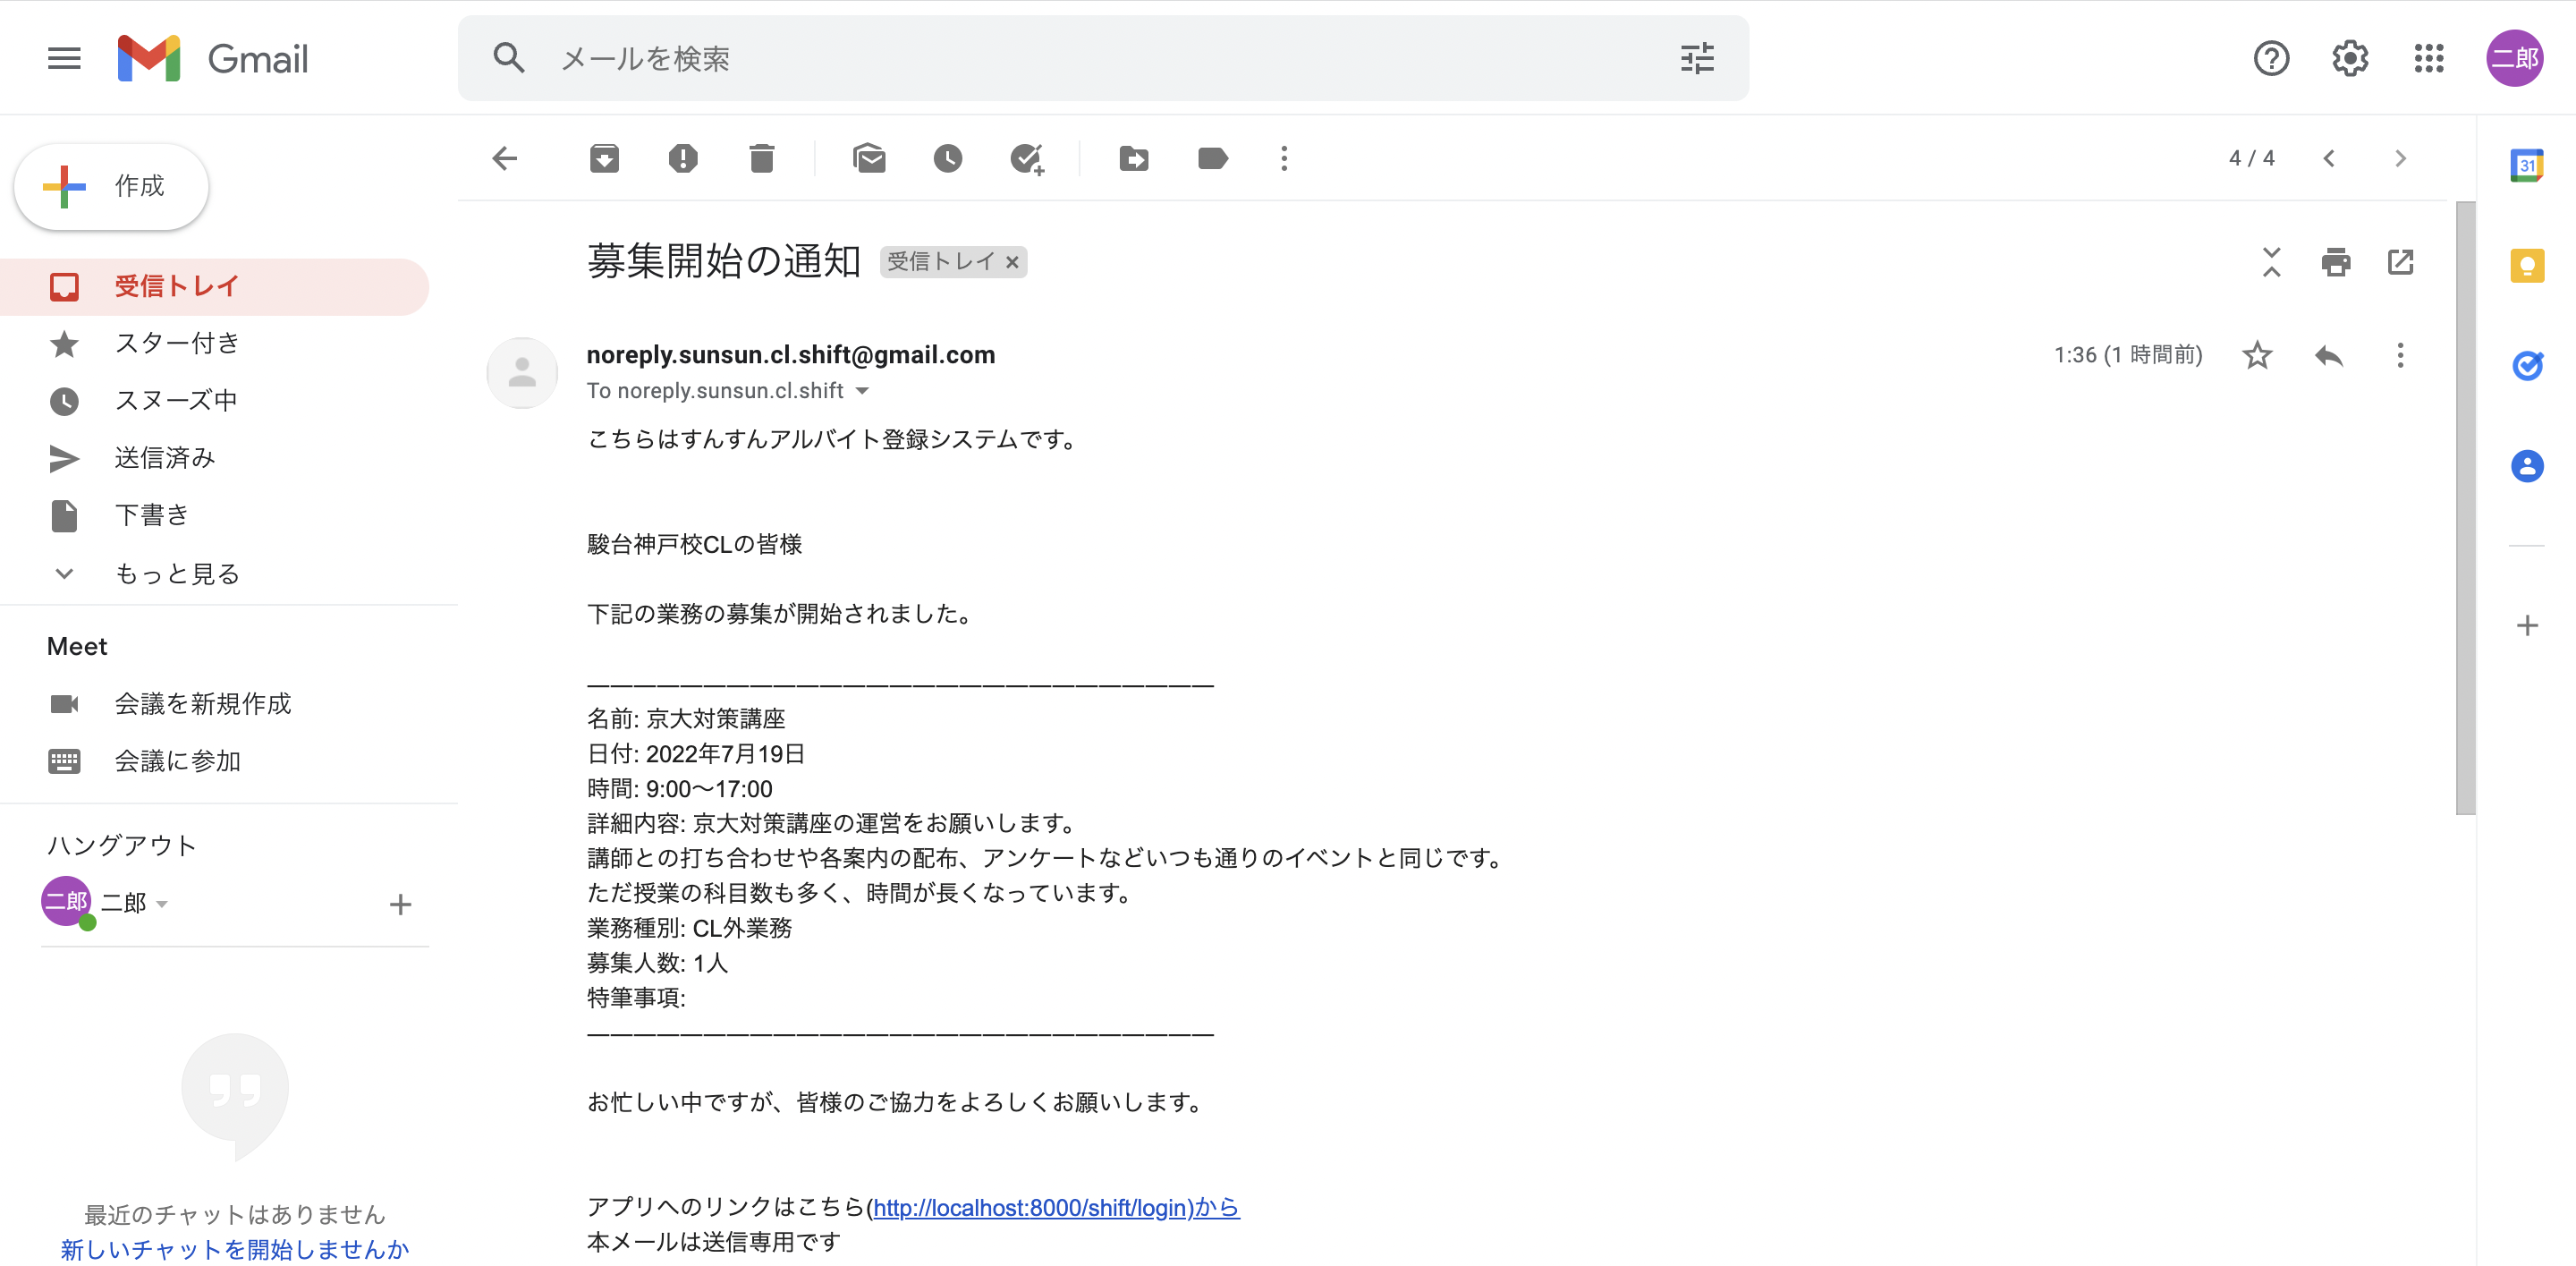
\includegraphics[width=0.8\linewidth]{../figure/14_mail_2.png}
				}
		\end{figure}
		3日前までに応募者数が定員に達しなかった業務について、このメールが全従業員宛にBCCで送信されます。

\end{document}
